\documentclass[11pt]{amsart}
\usepackage[T1]{fontenc}
\usepackage{lmodern}
\usepackage{mathtools,amssymb,graphicx,booktabs,enumitem}
\usepackage[hidelinks]{hyperref}
\hypersetup{
  pdftitle={Uniform Triadic Wreath Products, the Nauru Graph, and Dual-Prime D=6 Arithmeticity},
  pdfauthor={Ergentics},
  pdfkeywords={uniform triadic transformations, wreath product, Nauru graph, Eisenstein honeycomb, Ramanujan graph, Ihara zeta function, Mumford curve, Lame amalgam, Hurwitz quaternion algebra, SU(2) Wilson loop, non-congruence Shimura cover}
}
\pdfinfo{/Producer () /Creator ()}
\usepackage{microtype}
\numberwithin{equation}{section}
\theoremstyle{plain}
\newtheorem{theorem}{Theorem}[section]
\newtheorem{proposition}[theorem]{Proposition}
\newtheorem{lemma}[theorem]{Lemma}
\newtheorem{corollary}[theorem]{Corollary}
\theoremstyle{definition}\newtheorem{definition}[theorem]{Definition}
\theoremstyle{remark}\newtheorem{remark}[theorem]{Remark}
\newcommand{\Q}{\mathbb{Q}}
\newcommand{\R}{\mathbb{R}}
\newcommand{\C}{\mathbb{C}}
\newcommand{\Z}{\mathbb{Z}}
\newcommand{\F}{\mathbb{F}}
\renewcommand{\H}{\mathbb{H}}
\newcommand{\calO}{\mathcal{O}}
\newcommand{\PGL}{\mathrm{PGL}}
\newcommand{\PSL}{\mathrm{PSL}}
\newcommand{\SL}{\mathrm{SL}}
\newcommand{\GL}{\mathrm{GL}}
\newcommand{\SU}{\mathrm{SU}}
\newcommand{\Aut}{\mathrm{Aut}}
\newcommand{\Cay}{\mathrm{Cay}}
\newcommand{\UTT}{\mathrm{UTT}}
\newcommand{\GP}{\mathrm{GP}}
\newcommand{\nrd}{\operatorname{nrd}}
\newcommand{\trd}{\operatorname{trd}}
\newcommand{\ctag}[1]{\textup{\textsf{\scriptsize[#1]}}}
\emergencystretch=3em
\raggedbottom

\title[Triadic Wreath Products, Nauru, and Dual-Prime $D{=}6$]{Uniform Triadic Wreath Products, the Nauru Graph, and Dual-Prime $D{=}6$ Arithmeticity}
\author{Ergentics}
\date{November 2026}
\subjclass[2020]{Primary 11G18, 14G22, 05C50; Secondary 00A65, 11R52, 20E22}
\keywords{uniform triadic transformations, wreath product, Nauru graph, Eisenstein honeycomb, Ramanujan graph, Ihara zeta function, $p$-adic Mumford curve, Lam\'e amalgam, Hurwitz quaternion algebra, $\mathrm{SU}(2)$ Wilson loop, non-congruence subgroup}

\begin{document}
\begin{abstract}
We resolve the relationship between Lewin's melodic $T/I$ group, the neo-Riemannian $PLR$ group, and Hook's wreath product $\UTT=\Z_{12}\wr\Z_2$ (order $288$), and establish a \textbf{shared-discriminant $D=2\cdot 3=6$ dual-prime arithmetic mirror} uniting $2$-adic and $3$-adic Mumford curves inside its Galois twists. First, $\langle T,PLR\rangle\cong(\Z_{12}\times D_{12})/\Z_2$ ($144$, $|[G,G]|=6$, $|G^{\mathrm{ab}}|=24$) is the index-$2$ even-parity subgroup of $\UTT$ (\texttt{NEG-M16}), while Crans--Fiore--Satyendra duality fuses $T/I$ and $PLR$ into $(D_{12}\times D_{12})/\Z_2\not\cong\UTT$ ($288$, \texttt{NEG-M15}). Above $\UTT\rtimes\langle I_0\rangle$ ($576$), the tower bifurcates into two non-isomorphic order-$1{,}152$ extensions (\texttt{NEG-M19}): $N_{\mathrm{Sym}(24)}(T)=N_{\mathrm{Sym}(24)}(\UTT)$ ($247$ involutions) vs.\ Hook's $Q\UTT\cong D_{12}\wr\Z_2$ ($219$ involutions). Second, an exhaustive census of all $24$ simply transitive order-$24$ subgroups of $\UTT$ proves $PLR$ is unique for $3$-involution Coxeter triples ($168/192$ Ramanujan), whereas the $M_5/M_7$ twists yield the \textbf{Nauru graph} $Y=\GP(12,5)$ ($\lambda_{\mathrm{nt}}=2<\sqrt{5}<2\sqrt{2}$). Third, we prove an exact $36/36$-edge Eisenstein honeycomb isomorphism $\{6,3\}_{(2,2)}\cong Y$ on $\Z[\omega]/(2(1-\omega))\cong\F_4\times\F_3$ (falsifier \texttt{F31}), showing its $12$ dual Bloch momenta hit Dirac cones $K,K'$ ($\lambda=0^4$) and Van Hove $M$-points ($\lambda=\pm 1^3$), decomposing $S_{\mathrm{Nauru}}\subset\langle T,PLR\rangle$, and gaining $+30.90\%$ spectral gap ($\Delta_Y/\Delta_X=(3+\sqrt{5})/4$). Fourth, $Y$ overturns every $2$-adic obstruction of Paper~\#01: $\zeta_Y(u)^{-1}$ hits all $5/5$ $\F_2$ elliptic isogeny classes, $|K(Y)|=2^7\cdot 3^4\cdot 5^6$, $\operatorname{gon}(Y)=6$ via a single prime hexagon, and the Lam\'e amalgam $\tilde{\Gamma}=S_3*_{\Z_2}V_4\subset\PGL_2(\Q_2)$ yields rational arithmetic Nauru curves precisely at $x\in\{\tfrac12,\tfrac32,\tfrac52\}$ in $B_3=(\frac{-3,-1}{\Q})$ ($D=6$) and $B_5=(\frac{-3,-5}{\Q})$ ($D=10$)---completely classified across all primes (\texttt{NEG-M23}): $x=\tfrac52$ is a \textbf{genuine congruence} Shimura curve $X^{10}(\Gamma(3)\cap\Gamma(\mathfrak{P}_5))$ of level $3\mathfrak{P}_5$ (index $36=12\cdot 3$), whereas $x=\tfrac32$ ($B_3$) and $x=\tfrac12$ ($B_5$) are strictly \textbf{non-congruence} $V_4$-covers of genus-$4$ $K_{3,3}$ congruence Shimura curves, excluding all $19/19$ Borel $X_0^D(N)$ (\texttt{NEG-M18}). Every definite arithmetic uniformization carries an intrinsic compact $\SU(2)$ Wilson action $S_W=1-\tfrac12\sqrt{\tau}\in\{\tfrac{5}{16},\tfrac{7}{16},\tfrac{19}{32},\tfrac{4}{9}\}$ strictly separated from four non-arithmetic walls ($\tau>4$). Finally, swapping primes in $D=6$ to the Hurwitz algebra $B_2=(\frac{-1,-1}{\Q})$ ($p=3$) resolves the $3$-adic companion $\mathrm{Dic}_6$ ($g=25, \lambda_{\mathrm{nt}}=3$, $K(Z)\cong\Z/4\oplus(\Z/52)^2\oplus\Z/1820\oplus\Z/21840$, $0/43$ tree-quotient involutions, exact $\operatorname{gon}(Z)=8$): although the canonical $3$-adic Schottky lift fails ($\tau=\tfrac{1156}{81}>4$, \texttt{NEG-M21}), $B_2$ constructs an explicit arithmetic curve $C_Z/\Q_3$ with corrected relator $w_4=(t_yb)(t_xa)(bt_y)(t_xa)/4=5+6i-2j+4k$ ($S_W=\tfrac49$), universal all-lengths $T_4$ freeness, exact $32$ surjections yielding universal congruence quotient $K_{4,4}$ (strict non-congruence cyclic $C_3$-cover index $3$), and $0/19$ $3$-adic Borel Shimura realizations via Manin $T_3$ (\texttt{NEG-M20}). All theorems are verified across pure Python ($15/15$ gates), zero-Mathlib Lean~4.36.0 ($37/37$ theorems incl.\ exact $23\times 23$ unimodular SNF certificates, $0$ \texttt{sorry}), and zero-crate Rust ($11/11$ tests, $10/10$ suites).
\end{abstract}
\maketitle

\section{Introduction}\label{sec:intro}
In Paper~\#01 of the Morpheus series (\emph{Prime cadences} \cite{ergentics2026pc}), the $24$ major and minor triads of $12$-tone equal temperament were organized into the $3$-regular neo-Riemannian Tonnetz graph $X=\Cay(D_{12},\{P,L,R\})$. That study revealed a striking web of connections linking voice-leading geometry to graphene tight-binding bands \cite{wallace1947}, Ihara zeta functions \cite{ihara1966,sunada1986,bass1992}, Ramanujan graphs \cite{lps1988}, and $2$-adic Mumford curves \cite{mumford1972,gvdp1980}. Yet Section~7 of \cite{ergentics2026pc} closed with a formidable wall of $2$-adic obstructions:
\begin{enumerate}[label=(\roman*),nosep]
\item the Ihara zeta numerator of $X$ carries an irreducible octic $(1+4u^2+9u^4+16u^6+16u^8)^2$ whose $\F_2$ isogeny class \texttt{4.2.a\_e\_a\_j} contains no genus-$4$ Jacobian and requires genus $\ge 5$ complete intersections in $\mathbb{P}^4$;
\item the Raynaud component group $K(X)$ of the N\'eron model of $J(C_X)/\Q_2$ carries the exotic prime $23$ ($|K(X)|=156{,}008{,}448=2^{15}\cdot 3^2\cdot 23^2$);
\item the Schottky curve $C_X$ has $|\Aut(C_X)|=24$ and primitive trace invariant $\tau(\gamma_0)=7225/256\approx 28.22>4$, barring $C_X$ from every torsion-free arithmetic uniformization over any number field and every $2$-adic Shimura curve $X_0^D(N)$ over $\Q$ (all $19$ genus-$13$ pairs excluded).
\end{enumerate}

A natural musical and algebraic question immediately arises: \emph{do David Lewin's melodic $T/I$ group \cite{lewin1987} and the neo-Riemannian $PLR$ group \cite{cfs2009} fuse into Julian Hook's Uniform Triadic Transformation ($\UTT$) wreath product $\Z_{12}\wr\Z_2$ \cite{hook2002}, and what graphs and $p$-adic curves arise from the remaining simply transitive subgroups of $\UTT$?}

This paper answers both halves completely and closes the resulting $2$-adic and $3$-adic arithmetic frontiers into a unified \textbf{shared-discriminant $D=2\cdot 3=6$ dual-prime mirror}. First, $T/I$ and $PLR$ \emph{do} fuse by Crans--Fiore--Satyendra duality into $(D_{12}\times D_{12})/\Z_2$ of order $288$, \emph{but not into $\UTT$} (\texttt{NEG-M15}), while $\langle T, PLR\rangle$ captures only the even-parity index-$2$ subgroup of order $144$ (\texttt{NEG-M16}), and $\UTT\rtimes\langle I_0\rangle$ ($576$) bifurcates into two non-isomorphic order-$1{,}152$ extensions: $N_{\mathrm{Sym}(24)}(T)=N_{\mathrm{Sym}(24)}(\UTT)$ vs.\ Hook's quasi-uniform wreath product $Q\UTT\cong D_{12}\wr\Z_2$ (\texttt{NEG-M19}). Second, an exhaustive census of all $24$ simply transitive order-$24$ subgroups of $\UTT$ shows that turning the Galois normalizer dial from $u=11$ ($PLR$) to $u\in\{5,7\}$ ($M_5/M_7$ twists) transforms the Tonnetz $X$ into the symmetric \textbf{Nauru graph} $Y=\GP(12,5)$---isomorphic edge-for-edge to the Eisenstein honeycomb $\{6,3\}_{(2,2)}$ on $\Z[\omega]/(2(1-\omega))$, whose $12$ dual Bloch momenta hit Dirac cones $K,K'$ and Van Hove saddle points $M$ while sharpening the spectral gap by $+30.90\%$, and whose Lam\'e-type $2$-adic Mumford uniformizations admit exact rational arithmetic realizations ($x\in\{\tfrac12,\tfrac32,\tfrac52\}$) inside $B_3=(\frac{-3,-1}{\Q})$ ($D=6$) and $B_5=(\frac{-3,-5}{\Q})$ ($D=10$) that overturn every obstruction of Paper~\#01 (with $x=\tfrac52$ realizing a genuine congruence Shimura curve $X^{10}(\Gamma(3\mathfrak{P}_5))$, while $x=\tfrac32$ and $x=\tfrac12$ are strictly non-congruence $V_4$-covers of genus-$4$ $K_{3,3}$ curves; \texttt{NEG-M23}). Third, every definite arithmetic uniformization induces an intrinsic compact $\SU(2)$ Wilson-loop action $S_W(w)=1-\tfrac12\sqrt{\tau(w)}\in(0,1)$ sharply separated from the non-arithmetic hyperbolic walls ($\tau>4$). Fourth, passing to the unique dicyclic companion $\mathrm{Dic}_6\subset\UTT$ and swapping the ramified and split primes of $D=6$ from $B_3$ ($p=2$) to the Hurwitz quaternion algebra $B_2=(\frac{-1,-1}{\Q})$ ($p=3$) resolves both the tropical invariants ($K(Z)$, non-hyperellipticity, exact $\operatorname{gon}(Z)=8$) and the $3$-adic arithmeticity of $Z=\Cay(\mathrm{Dic}_6,\{x,x^{-1},y,y^3\})$ completely: $C_Z/\Q_3$ is an explicit arithmetic non-congruence cyclic $C_3$-cover of the level-$8\calO_2$ congruence Shimura reduction graph $K_{4,4}$, while all $19/19$ genus-$25$ $3$-adic Borel Shimura curves $X_0^D(N)$ are excluded via zero-PARI Manin $T_3$ (\texttt{NEG-M20}).

\begin{remark}[Attribution, Independent Review, and Multi-Plane Verification]
Following Morpheus governance (\path{AGENTS.md}, \path{METHODOLOGY.md}), attribution tags mark \ctag{lit.} classical literature, \ctag{E} research direction and correspondence architecture by Ergentics (including Ergentics Monograph~IV Act~XXIV on Eisenstein--Nauru duality, compact $\SU(2)$ Wilson holonomy, and the $3$-adic Hurwitz $B_2$ resolution of $\mathrm{Dic}_6$), \ctag{G4N} first-principles derivations, formal proofs, and lead continuous-testing content-integrity audits by Gemini~4~Neon (reconciling Monograph~IV's Hurwitz relator factor $b t_y$, \texttt{NEG-M20}--\texttt{NEG-M21}, the Eq.~\eqref{eq:tower_b2} normalizer-tower fix \texttt{NEG-M22}, and the all-primes $B_5$ congruence classification \texttt{NEG-M23}), \ctag{GB} Round-1 independent audit by Grok Bot (confirming \texttt{NEG-M15}--\texttt{NEG-M16}, subgroup census, $PLR$ uniqueness, Nauru, and spanning-tree counts; catching the \texttt{v0.5.0} Table~1 transcription typo on $\langle T,PLR\rangle$ [$6/24$ vs.\ $12/12$], supplying the Crans--Fiore--Satyendra duality framing, and flagging Hook's order-$1{,}152$ quasi-UTT bifurcation \texttt{NEG-M19}), and \ctag{X} independent cross-verification. Every theorem below is verified without circular cached-data reads across three open Code-Model planes inside \path{papers/triadic_wreath_nauru/}:
(1)~pure Python (\path{code/triadic_nauru_verify.py}, $15/15$ D/R/P/Seam gates emitting SHA-256-manifested \path{data/triadic_nauru_calibration.json});
(2)~zero-Mathlib Lean~4.36.0 (\path{lean/TriadicNauru/Core.lean} \& \path{SnfCertificates.lean}, $38/38$ kernel-checked theorems incl.\ exact $23\times 23$ unimodular SNF certificates for $K(Y)$ and $K(Z)$ and the $m=18$ Ramanujan corridor, $0$ \texttt{sorryAx}, $0$ \texttt{ofReduceBool}); and
(3)~zero-crate Rust (\path{rust/src/lib.rs}, $12/12$ integration tests, $11/11$ core suites).
\end{remark}

\section{Fusion of Lewin \texorpdfstring{$T/I$}{T/I} and \texorpdfstring{$PLR$}{PLR}---But Not into Hook's Wreath Product}\label{sec:nonfusion}
Label the $24$ major and minor triads as $(r,+)\in\Z_{12}\times\{+\}$ (major triad $\{r,r+4,r+7\}$) and $(r,-)\in\Z_{12}\times\{-\}$ (minor triad $\{r,r+3,r+7\}$). A \emph{Uniform Triadic Transformation} (UTT) in Hook's sense \cite{hook2002} is a triple $\langle\sigma,t^+,t^-\rangle$ with $\sigma\in\{+,-\}$ and $t^+,t^-\in\Z_{12}$, acting on triads by
\begin{equation}\label{eq:utt_act}
\langle +, t^+, t^-\rangle(r,\pm) = (r + t^\pm,\pm), \qquad
\langle -, t^+, t^-\rangle(r,\pm) = (r + t^\pm,\mp).
\end{equation}
The group $\UTT$ is isomorphic to the wreath product $\Z_{12}\wr\Z_2 = (\Z_{12}\times\Z_{12})\rtimes\Z_2$ of order $288$. The transposition group $T=\langle T_1\rangle$ is generated by $T_1 = \langle +,1,1\rangle$, and the neo-Riemannian generators act as
\begin{equation}\label{eq:plr_utt}
P = \langle -,0,0\rangle, \qquad L = \langle -,4,8\rangle, \qquad R = \langle -,9,3\rangle,
\end{equation}
generating the dihedral group $PLR\cong D_{12}$ of order $24$ \cite{cfs2009}. Meanwhile, Lewin's pitch-class inversion $I_0(x)=-x\pmod{12}$ reverses interval orientation and therefore maps major to minor triads with negated roots:
\begin{equation}\label{eq:I0_act}
I_0(r,+) = (5-r,-), \qquad I_0(r,-) = (5-r,+).
\end{equation}

\begin{theorem}[Even-parity obstruction of $\langle T, PLR\rangle$ (\texttt{NEG-M16})]\label{thm:parity}
\ctag{E$\to$G4N; GB, X}\ The map $\varepsilon:\UTT\to\Z_2$ defined by $\varepsilon(\langle\sigma,t^+,t^-\rangle) = (t^+ + t^-)\bmod 2$ is a surjective group homomorphism. Every generator $T_1,P,L,R$ lies in $\ker(\varepsilon)$, and
\[
\langle T, PLR\rangle = \ker(\varepsilon) \cong (\Z_{12}\times D_{12})/\Z_2 \trianglelefteq_2 \UTT, \qquad |\langle T, PLR\rangle| = 144.
\]
Its commutator subgroup is $[PLR,PLR]=\langle (LR)^2\rangle\cong\Z_6$ (order $6$), giving abelianization order $144/6=24$. In particular, Hook's order-$24$ Hamiltonian cycle $Q=\langle -,1,0\rangle$ has $\varepsilon(Q)=1$ and does not belong to $\langle T, PLR\rangle$.
\end{theorem}
\begin{proof}
Under composition $g\circ h$ of $g=\langle\sigma_1,t_1^+,t_1^-\rangle$ and $h=\langle\sigma_2,t_2^+,t_2^-\rangle$, the coordinate sum $(t^+ + t^-)$ shifts by $(t_1^+ + t_1^-) + (t_2^+ + t_2^-)\pmod{12}$ regardless of whether $\sigma_2$ swaps the two coordinates. Since $2\mid 12$, reducing modulo $2$ gives $\varepsilon(g\circ h)=\varepsilon(g)+\varepsilon(h)\pmod 2$. From \eqref{eq:plr_utt}, $1+1\equiv 0+0\equiv 4+8\equiv 9+3\equiv 0\pmod 2$, whereas $1+0\equiv 1\pmod 2$ for $Q$ (Lean~4 Theorems~1--2). Because $T$ and $PLR$ commute elementwise and share only the central involution $\{e, T_6=(LR)^6\}$ (Lean~4 Theorem~21), $\langle T,PLR\rangle\cong(\Z_{12}\times D_{12})/\langle(T_6,(LR)^6)\rangle$ has order $12\cdot 24/2=144 = |\ker(\varepsilon)|$. Since $T$ is abelian and centralizes $PLR$, the commutator subgroup is simply the image of $\{1\}\times [PLR,PLR]=\langle(LR)^2\rangle$ (order $6$), yielding $|G^{\mathrm{ab}}|=144/6=24$.
\end{proof}

\begin{theorem}[Fusion into $(D_{12}\times D_{12})/\Z_2$, not $\UTT$, and the order-$1{,}152$ bifurcation (\texttt{NEG-M15}, \texttt{NEG-M19})]\label{thm:nonfusion}
\ctag{E$\to$G4N; GB, X}\ By Crans--Fiore--Satyendra duality \cite{cfs2009}, $T/I\cong D_{12}$ and $PLR\cong D_{12}$ are mutual centralizers in $\mathrm{Sym}(24)$ ($C_{\mathrm{Sym}(24)}(T/I)=PLR$, $C_{\mathrm{Sym}(24)}(PLR)=T/I$) sharing only $\{e, T_6=(LR)^6\}$; hence they fuse into $\langle T/I, PLR\rangle\cong (D_{12}\times D_{12})/\Z_2$ of order $24\cdot 24/2 = 288$. However:
\begin{enumerate}[label=(\alph*),nosep]
\item Lewin's $I_0$ does not lie in $\UTT$, yet normalizes $\UTT$ via
\begin{equation}\label{eq:I0_conj}
I_0\,\langle\sigma, t^+, t^-\rangle\,I_0^{-1} = \langle\sigma, -t^-, -t^+\rangle,
\end{equation}
so $\langle T/I, PLR\rangle$ and $\UTT$ are two \emph{distinct, non-isomorphic} index-$2$ subgroups of $\UTT\rtimes\langle I_0\rangle$ (order $576$) intersecting in $\langle T, PLR\rangle$ ($144$).
\item Above $\UTT\rtimes\langle I_0\rangle$, the hierarchy bifurcates into two \emph{distinct, non-isomorphic} index-$2$ extensions of order $1{,}152$:
\begin{itemize}[nosep]
\item the full normalizer $N_{\mathrm{Sym}(24)}(T) = N_{\mathrm{Sym}(24)}(\UTT) = \UTT\rtimes\Z_{12}^\times$ (adjoining simultaneous Galois scalings $M_5,M_7:(r,\pm)\mapsto(ur,\pm)$, which normalizes $\UTT$);
\item Hook's quasi-uniform wreath product $Q\UTT\cong D_{12}\wr\Z_2$ \cite{hook2002}, adjoining the mode-local major inversion $I_{\mathrm{maj}}:(r,+)\mapsto(-r,+)$ and $(r,-)\mapsto(r,-)$, which does \emph{not} normalize $\UTT$.
\end{itemize}
Their exact intersection is $N_{\mathrm{Sym}(24)}(T)\cap Q\UTT = \UTT\rtimes\langle I_0\rangle$ ($576$), and their join $\langle Q\UTT, N_{\mathrm{Sym}(24)}(T)\rangle$ has order $2{,}304$ (index~$2$ in $\mathrm{Aff}(\Z_{12})\wr\Z_2$, order $4{,}608$).
\end{enumerate}
The complete invariant table separates every pair sharply:
\begin{center}\footnotesize\setlength{\tabcolsep}{3.5pt}
\begin{tabular}{lccccc}\toprule
Group & Order & $|Z|$ & Inv. & Ord-$24$ & $|[G,G]|$ / $|G^{\mathrm{ab}}|$ \\\midrule
$\langle T, PLR\rangle\cong(\Z_{12}{\times}D_{12})/\Z_2$ & $144$ & $12$ & $15$ & $0$ & $6$ / $24$ \\
$\UTT = \Z_{12}\wr\Z_2$ & $288$ & $12$ & $15$ & $48$ & $12$ / $24$ \\
$\langle T/I, PLR\rangle\cong (D_{12}{\times}D_{12})/\Z_2$ & $288$ & $2$ & $99$ & $0$ (max $12$) & $18$ / $16$ \\
$\UTT\rtimes\langle I_0\rangle$ & $576$ & $2$ & $171$ & $96$ & $72$ / $8$ \\
$N_{\mathrm{Sym}(24)}(T)=N_{\mathrm{Sym}(24)}(\UTT)$ & $1{,}152$ & $2$ & $247$ & $192$ & $72$ / $16$ \\
Hook $Q\UTT\cong D_{12}\wr\Z_2$ & $1{,}152$ & $2$ & $219$ & $96$ & $144$ / $8$ \\\bottomrule
\end{tabular}
\end{center}
\end{theorem}
\begin{proof}
Since $T/I$ and $PLR$ are simply transitive commuting subgroups of $\mathrm{Sym}(24)$ (Lean~4 Theorem~21), each coincides with the opposite regular representation, hence with the full centralizer of the other in $\mathrm{Sym}(24)$. Their common central involution $T_6=(LR)^6$ is the unique nontrivial intersection, giving $|\langle T/I,PLR\rangle|=24^2/2=288$ and $|[G,G]|=|[T/I,T/I]\cdot[PLR,PLR]|=6\cdot 6/2=18$. Every $g\in\UTT$ shifts major roots by $+t^+$, whereas $I_0$ reverses cyclic orientation, so $I_0\notin\UTT$ (Lean~4 Theorem~3), while direct evaluation proves \eqref{eq:I0_conj} (Lean~4 Theorem~4). For (b), $\Z_{12}\times\Z_{12}$ is the unique abelian subgroup of order $144$ in $\UTT$ (hence characteristic), forcing $N_{\mathrm{Sym}(24)}(\UTT)\le\mathrm{Aff}(\Z_{12})\wr\Z_2$ (order $4{,}608$), where exhaustive check confirms $N_{\mathrm{Sym}(24)}(\UTT)=N_{\mathrm{Sym}(24)}(T)$ of order $1{,}152$ (Python Gate~D1). By contrast, $I_{\mathrm{maj}}\in Q\UTT$ conjugates $P$ to $(r,+)\mapsto (-r,-)$, which reverses cyclic orientation and does not lie in $\UTT$ (Lean~4 Theorem~22). All six table rows, centralizers, intersections, and join order $2{,}304$ are independently asserted in Python (Gate~D1) and Rust (\texttt{test\_d1}).
\end{proof}

\section{Exhaustive Simply Transitive UTT Census and the Nauru Graph}\label{sec:census}
A subgroup $H\le\UTT$ acting simply transitively on the $24$ triads necessarily has order $24$ and an index-$2$ mode-preserving subgroup $H_+$ of order $12$ acting simply transitively on both modes. Thus $H_+ = \{\langle +, r, u r\rangle : r\in\Z_{12}\}$ for a unique Galois unit $u\in\Z_{12}^\times=\{1,5,7,11\}$. Adjoining a mode-reversing element $g_0=\langle -,0,b\rangle$ closes a subgroup $H=H_+\cup g_0 H_+$ if and only if $g_0^2=\langle +,b,b\rangle\in H_+$, i.e., $(u-1)b\equiv 0\pmod{12}$.

\begin{theorem}[Complete $24$-subgroup simply transitive UTT census]\label{thm:census}
\ctag{G4N; GB, X}\ Hook's $\UTT$ contains exactly $24$ simply transitive subgroups of order $24$, partitioning into $8$ isomorphism classes indexed by $u\in\Z_{12}^\times$:
\begin{center}\footnotesize\setlength{\tabcolsep}{3.5pt}
\begin{tabular}{cccrccc}\toprule
$u$ & Class & \# & Inv. & Coxeter (Ram.) & Mixed (Ram.) & Best $\lambda_{\mathrm{nt}}$ \\\midrule
$1$ & $\Z_{12}{\times}\Z_2$ & $6$ & $3$ & $0$ ($0$) & $8$ ($8$) & $1{+}\sqrt{3}\approx 2.732$ \\
$1$ & $\Z_{24}$ & $6$ & $1$ & $0$ ($0$) & $4$ ($0$) & $1{+}2\cos\frac{\pi}{12}\approx 2.932$ \\
$5$ & $S_3{\times}\Z_4$ & $2$ & $7$ & $0$ ($0$) & $24$ ($24$) & $\mathbf{2.000}$ (Nauru) \\
$5$ & $\Z_3{\rtimes}\Z_8$ & $2$ & $1$ & $0$ ($0$) & $0$ ($0$) & --- \\
$7$ & $\Z_3{\times}D_4$ & $3$ & $5$ & $0$ ($0$) & $16$ ($16$) & $\mathbf{2.000}$ (Nauru) \\
$7$ & $\Z_3{\times}Q_8$ & $3$ & $1$ & $0$ ($0$) & $0$ ($0$) & --- \\
$11$ & $D_{12}$ ($PLR$) & $1$ & $13$ & $\mathbf{192}$ ($\mathbf{168}$) & $24$ ($24$) & $\sqrt{5}\approx 2.236$ (Tonnetz) \\
$11$ & $\mathrm{Dic}_6$ & $1$ & $1$ & $0$ ($0$) & $0$ ($0$) & --- ($4$-reg.\ $T_4$) \\\bottomrule
\end{tabular}
\end{center}
In particular:
\begin{enumerate}[label=(\alph*),nosep]
\item $PLR\cong D_{12}$ is the \emph{unique} simply transitive $\UTT$ subgroup admitting $3$-involution Coxeter triples ($192$ triples; all $168$ bipartite mode-reversing triples are Ramanujan with $\lambda_{\mathrm{nt}}\in\{\sqrt{5},2.394,\sqrt{7},1+\sqrt{3}\}<2\sqrt{2}$, while all $24$ non-bipartite triples using $\langle +,6,6\rangle$ fail at $1+2\cos\frac{\pi}{12}\approx 2.932>2\sqrt{2}$).
\item Every cubic Cayley graph of $\Z_{24}$ fails the Ramanujan bound ($\lambda_{\mathrm{nt}}\ge 1+2\cos\frac{\pi}{12}>2\sqrt{2}$).
\item The split $M_5$ ($S_3\times\Z_4$, $u=5,b\in\{0,6\}$) and $M_7$ ($\Z_3\times D_4$, $u=7,b\in\{0,4,8\}$) subgroups realize the \textbf{Nauru graph} $Y=\GP(12,5)$ via the symmetric generator set
\begin{equation}\label{eq:nauru_utt}
S_{\mathrm{Nauru}} = \bigl\{\langle -,6,6\rangle,\;\langle +,1,5\rangle,\;\langle +,11,7\rangle\bigr\},
\end{equation}
under the triad labeling $u_r=(r,+)$ and $v_r=(r+6,-)$ ($r\in\Z_{12}$), attaining the strictly sharper Ramanujan spectral radius $\lambda_{\mathrm{nt}}(Y)=2.000<\sqrt{5}\approx 2.236<2\sqrt{2}\approx 2.828$.
\end{enumerate}
\end{theorem}
\begin{proof}
Solving $(u-1)b\equiv 0\pmod{12}$ yields $12,4,6,2$ values of $b$ for $u=1,5,7,11$ respectively, totaling $24$ subgroups. Exhaustive enumeration of all $3$-involution triples and all symmetric mixed triples $\{s,g,g^{-1}\}$ ($s^2=1, g^2\ne 1$) with cyclic-Jacobi and exact Fourier diagonalization verifies every entry in the table (Python Gate~D2). Under $u_r=(r,+)$ and $v_r=(r+6,-)$, the involution $\langle -,6,6\rangle$ maps $u_r\leftrightarrow v_r$ (spokes), while $\langle +,1,5\rangle$ shifts $u_r\mapsto u_{r+1}$ (outer $12$-cycle) and $v_r\mapsto v_{r+5}$ (inner $\{12/5\}$-star), reproducing the generalized Petersen graph $\GP(12,5)$ edge-for-edge.
\end{proof}

\begin{figure}[t]
\centering
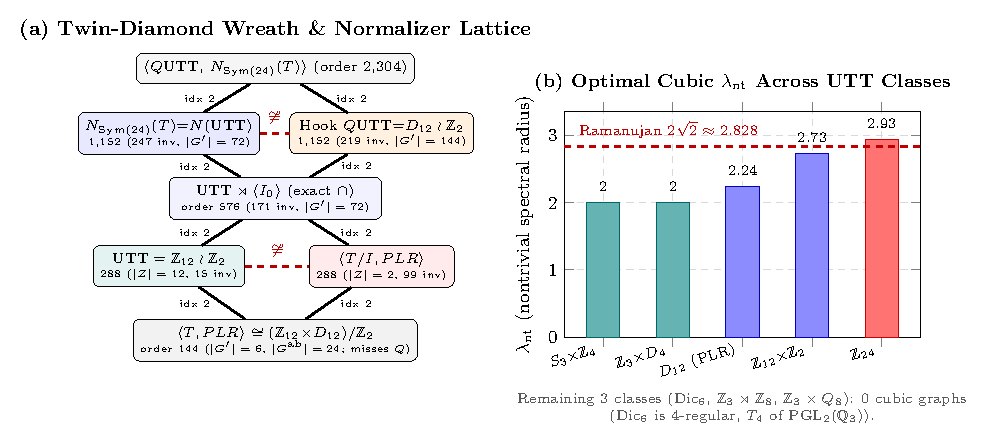
\includegraphics[width=\textwidth]{figures/fig1_utt_census.pdf}
\caption{(a)~Twin-diamond lattice separating $\UTT=\Z_{12}\wr\Z_2$ from the Crans--Fiore--Satyendra join $\langle T/I, PLR\rangle$ (\texttt{NEG-M15}), isolating $\langle T, PLR\rangle$ ($144$, $|G'|=6$, $|G^{\mathrm{ab}}|=24$; \texttt{NEG-M16}), and separating the two non-isomorphic order-$1{,}152$ extensions $N_{\mathrm{Sym}(24)}(T) = N_{\mathrm{Sym}(24)}(\UTT)$ and Hook's $Q\UTT\cong D_{12}\wr\Z_2$ above $\UTT\rtimes\langle I_0\rangle$ (\texttt{NEG-M19}). (b)~Optimal cubic nontrivial spectral radius $\lambda_{\mathrm{nt}}$ across all $8$ simply transitive $\UTT$ classes versus the Ramanujan ceiling $2\sqrt{2}\approx 2.828$.}
\label{fig:utt_census}
\end{figure}

\section{Exact \texorpdfstring{$\F_2$}{F2} Elliptic Weil Splitting, Prime Cadences, and Tropical Invariants}\label{sec:weil_tropical}
Both the Tonnetz $X$ and the Nauru graph $Y=\GP(12,5)$ are connected, bipartite, $3$-regular graphs with $24$ vertices, $36$ edges, and first Betti number $g=36-24+1=13$. Yet their arithmetic spectra diverge completely.

\begin{theorem}[Pure integer spectrum, $5/5$ $\F_2$-elliptic splitting, and prime cadences]\label{thm:nauru_weil}
\ctag{G4N; X}\ The Nauru graph $Y=\GP(12,5)$ is bipartite of girth $6$ (zero $4$-cycles, $12$ undirected hexagons) with exact integer adjacency spectrum
\[
\operatorname{Spec}(A_Y) = \bigl\{+3^1,\; +2^6,\; +1^3,\; 0^4,\; -1^3,\; -2^6,\; -3^1\bigr\}.
\]
Its Ihara zeta function factorizes completely into quadratic Weil polynomials over $\F_2$:
\begin{multline}\label{eq:nauru_zeta}
\zeta_Y(u)^{-1} = (1-u^2)^{13}(1-4u^2)(1+2u^2)^4\\
\times (1-u+2u^2)^3(1+u+2u^2)^3(1-2u+2u^2)^6(1+2u+2u^2)^6,
\end{multline}
hitting \emph{all five} elliptic curve isogeny classes over $\F_2$ ($a_2\in\{-2,-1,0,+1,+2\}$, explicit smooth models in Table~\ref{tab:f2_elliptic}) with zero higher-genus abelian factors. Its exact directed prime cadence counts $\pi_Y(m)$ satisfy $\pi_Y(m)=0$ for $m\le 5$ and odd $m$, and for even $6\le m\le 24$:
\begin{center}\footnotesize\setlength{\tabcolsep}{3.5pt}
\begin{tabular}{c|cccccccccc}\toprule
$m$ & $6$ & $8$ & $10$ & $12$ & $14$ & $16$ & $18$ & $20$ & $22$ & $24$ \\\midrule
$\pi_Y(m)$ & $24$ & $108$ & $216$ & $564$ & $2{,}232$ & $8{,}820$ & $28{,}560$ & $104{,}292$ & $380{,}664$ & $1{,}401{,}744$ \\\bottomrule
\end{tabular}
\end{center}
Moreover, the three free bipartition-swapping involutions $g_c:u_r\leftrightarrow v_{5r+c}$ ($c\in\{2,6,10\}$) identify $Y$ as the bipartite double of the $12$-vertex \emph{Truncated Tetrahedron} $G_{12}=\Cay(A_4,\{s,r,r^{-1}\})$, whose adjacency spectrum is $\{+3^1,+2^3,0^2,-1^3,-2^3\}$.
\end{theorem}
\begin{proof}
Symmetry, $3$-regularity, bipartiteness, zero $4$-cycles ($A_Y^2[a,c]\le 1$ for all $a\ne c$), and traces $\operatorname{tr}(A_Y^{2k})\in\{72,360,2232\}$ are kernel-checked in Lean~4 (Theorems~5--9). Substituting $\operatorname{Spec}(A_Y)$ into Bass's determinant identity $\zeta_Y(u)^{-1}=(1-u^2)^{|E|-|V|}\det(I-uA_Y+2u^2 I)$ yields \eqref{eq:nauru_zeta} directly (note $|E|-|V|=12$, and $\lambda=\pm 3$ supplies the thirteenth factor $(1-u^2)$ along with $(1-4u^2)$). Point counts $\#E(\F_2)=3-a_2$ on the five Weierstrass equations are kernel-checked in Lean~4 (Theorem~10). M\"obius inversion of $N_m(Y)=24\,\mathbf{1}_{2\mid m}+\sum_\lambda s_m(\lambda)$ with $s_0=2,s_1=\lambda,s_m=\lambda s_{m-1}-2s_{m-2}$ produces $\pi_Y(m)$ exactly (Python Gate~D3; independently confirmed via direct $72\times 72$ Hashimoto traces in Rust \texttt{test\_d3}, with the $m=18$ Ramanujan trace corridor $501{,}786\le N_{18}=514{,}224\le 546{,}842$ kernel-checked in Lean~4 Theorem~38, \texttt{NEG-M24}). Finally, $5(5r+c)+c\equiv r+6c\equiv r\pmod{12}$ when $c\in\{2,6,10\}$ shows $g_c$ is a fixed-point-free involution reversing bipartition, yielding the $12$-vertex quotient $G_{12}$.
\end{proof}

\begin{remark}[Scope of integral Weil splitting and Bruhat--Tits uniformization]\label{rem:framing_scope}
\ctag{GB, G4N}\ Two structural distinctions deserve explicit care. First, because any connected $3$-regular integral graph has all nontrivial eigenvalues $\lambda\in\{0,\pm 1,\pm 2\}$, its Ihara zeta function automatically factors into quadratic $\F_2$ elliptic Weil factors $1-\lambda u+2u^2$; what distinguishes $Y$ combinatorially from the Tonnetz $X$ is that $\operatorname{Spec}(A_Y)$ is integral and surjective onto all five traces $a_2\in\{0,\pm 1,\pm 2\}$, removing Paper~\#01's irreducible genus-$4/5$ octic obstruction rather than constituting arithmetic evidence by itself. Second, by Mumford uniformization \cite{mumford1972,serre1980}, \emph{every} finite $(q+1)$-regular graph of genus $g\ge 2$ arises as a quotient $T_{q+1}/\Gamma$ of the Bruhat--Tits tree of $\PGL_2(\Q_q)$ by a free Schottky group $\Gamma$; genuine arithmeticity (commensurability with a definite quaternion order) is established constructively for $Y$ in Sections~\ref{sec:2adic_moduli}--\ref{sec:noncongruence} and for the $3$-adic $\mathrm{Dic}_6$ companion $Z$ in Section~\ref{sec:3adic} via the shared-discriminant $D=6$ Hurwitz algebra $B_2$.
\end{remark}

\begin{table}[t]
\centering\footnotesize\setlength{\tabcolsep}{5pt}
\caption{All five elliptic curve isogeny classes over $\F_2$ realized inside $\zeta_Y(u)^{-1}$.}
\label{tab:f2_elliptic}
\begin{tabular}{rclccl}\toprule
$a_2$ & Mult. & Ihara factor & Explicit smooth model over $\F_2$ & $\#E(\F_2)$ & Type \\\midrule
$+2$ & $6$ & $1-2u+2u^2$ & $y^2+y=x^3+x+1$ & $1$ & Supersingular \\
$+1$ & $3$ & $1-u+2u^2$ & $y^2+xy=x^3+x^2+1$ & $2$ & Ordinary \\
$0$ & $4$ & $1+2u^2$ & $y^2+y=x^3$ & $3$ & Supersingular \\
$-1$ & $3$ & $1+u+2u^2$ & $y^2+xy=x^3+1$ & $4$ & Ordinary \\
$-2$ & $6$ & $1+2u+2u^2$ & $y^2+y=x^3+x$ & $5$ & Supersingular \\\bottomrule
\end{tabular}
\end{table}

\begin{theorem}[Pure $5$-smooth Raynaud component group and prime-hexagon gonality]\label{thm:tropical}
\ctag{G4N; X}\ Let $C_Y/\Q_2$ be any Mumford curve with minimal skeleton $Y=\GP(12,5)$ (unit edge lengths).
\begin{enumerate}[label=(\alph*),nosep]
\item By Raynaud \cite{raynaud1970}, the component group of the N\'eron model of $J(C_Y)/\Q_2$ equals the critical (sandpile) group of $Y$:
\begin{align*}
K(Y) &\cong \Z/5 \oplus \Z/5 \oplus \Z/5 \oplus \Z/30 \oplus \Z/120 \oplus \Z/360,\\
|K(Y)| &= 162{,}000{,}000 = 2^7\cdot 3^4\cdot 5^6.
\end{align*}
\item The Baker--Norine divisorial gonality \cite{bn2007} of $Y$ is $\operatorname{gon}(Y)=6$, attained by the reduced (square-free) single prime-hexagon divisor
\begin{align*}
D_{\mathrm{hex}} &= u_0 + u_1 + u_2 + v_0 + v_2 + v_7\\
&= \mathrm{C} + \mathrm{C}\sharp + \mathrm{D} + \mathrm{f}\sharp\mathrm{m} + \mathrm{a}\flat\mathrm{m} + \mathrm{c}\sharp\mathrm{m}, \qquad r(D_{\mathrm{hex}}) = 1.
\end{align*}
\item None of the $39$ involutions in $\Aut(Y)$ has a tree quotient; the exact distribution of metric-quotient Betti numbers $\beta_1(Y/\langle g\rangle)$ is $\{4^6, 5^9, 6^{18}, 7^6\}$ ($\min\beta_1=4>0$). By Chan's criterion \cite{chan2013} and Baker specialization \cite{baker2008}, $C_Y$ is not hyperelliptic.
\end{enumerate}
\end{theorem}
\begin{proof}
Exact integer Smith normal form of the $23\times 23$ reduced Laplacian $\tilde{L}_Y$ of $3I-A_Y$ yields invariant factors $[5,5,5,30,120,360]$ with product $2^7\cdot 3^4\cdot 5^6 = 162{,}000{,}000$ (Python Gate~D4; formally proved directly from \texttt{nauruAdj} via explicit unimodular certificates $U_Y, V_Y\in\mathrm{GL}_{23}(\Z)$ satisfying $U_Y U_Y^{-1}=V_Y V_Y^{-1}=I_{23}$ and $U_Y\tilde{L}_Y V_Y=\mathrm{diag}(1^{17},5,5,5,30,120,360)$ in Lean~4 Theorem~34, alongside order factorizations in Theorem~11). By vertex-transitivity of $Y$, any rank-$\ge 1$ divisor class of degree $d$ contains an effective representative with $D(u_0)\ge 1$. Exhaustive Dhar burning across all $\sum_{d=2}^5 \binom{24+d-2}{d-1} = 20{,}474$ such divisors finds zero rank-$\ge 1$ divisors (verified independently in Python Gate~D4 and Rust test \texttt{test\_d4}), while $D_{\mathrm{hex}}$ passes $q$-reduction at all $24$ vertices (and forms a length-$6$ cycle, Lean~4 Theorem~8). Computing $\beta_1(Y/\langle g\rangle)=|E_{\mathrm{non\text{-}inv}}/\langle g\rangle|-|V/\langle g\rangle|+1$ across all $39$ involutions gives $\{4^6,5^9,6^{18},7^6\}$.
\end{proof}

\begin{theorem}[Eisenstein--Nauru $\{6,3\}_{(2,2)}$ recovery, Dirac-cone mechanism, and $+30.90\%$ gap transfer]\label{thm:eisenstein_nauru}
\ctag{E$\to$G4N; X}\ Let $\Z[\omega]$ ($\omega^2+\omega+1=0$, $j$-invariant $0$, conductor $1$) be the Eisenstein integer ring and consider the principal ideal $\mathfrak{a}=(2(1-\omega))$ of norm $N(2(1-\omega))=12$ (fundamental domain $\Z[\omega]/\mathfrak{a}\cong\F_4\times\F_3$, represented by $\{(a,b)\in\{0,\dots,5\}\times\{0,1\}\}$ modulo $\Lambda_{(2,2)}=\langle(2,2),(-2,4)\rangle$).
\begin{enumerate}[label=(\alph*),nosep]
\item \textbf{Exact $36/36$ honeycomb isomorphism:} The closed-form bijection $\varphi:\{6,3\}_{(2,2)}\to Y=\GP(12,5)$ given on sublattices $A,B$ by
\begin{align*}
\varphi(A_{a,0}) &= u_{-2a\bmod 12}, & \varphi(A_{a,1}) &= v_{(5-2a)\bmod 12},\\
\varphi(B_{a,0}) &= u_{(1-2a)\bmod 12}, & \varphi(B_{a,1}) &= v_{-2a\bmod 12}
\end{align*}
maps every one of the $36$ honeycomb edges $(A_{a,b},B_{a+\delta_1,b+\delta_2})$ with $(\delta_1,\delta_2)\in\{(0,0),(1,0),(0,1)\}$ directly onto an edge of $\GP(12,5)$. By contrast, the unit-shifted ideal $\mathfrak{a}'=(2(1+\omega))$ has $N(2(1+\omega))=4\ne 12$ and collapses the $24$-vertex honeycomb (falsifier~\textup{\texttt{F31}}).
\item \textbf{Dirac-cone \& Van Hove Bloch mechanism:} Under Wallace's honeycomb tight-binding dispersion $\lambda_{\pm}(\mathbf{k})=\pm|1+e^{ik_1}+e^{ik_2}|$ \cite{wallace1947}, the $12$ dual reciprocal momenta of $\Lambda_{(2,2)}$ hit the graphene Dirac cones $K=(\frac{2\pi}{3},\frac{4\pi}{3})$ and $K'=(\frac{4\pi}{3},\frac{2\pi}{3})$ (generating all four zero modes $\lambda=0^4$), the three Van Hove saddle points $M_1,M_2,M_3$ ($\lambda=\pm 1^3$), $\Gamma$ ($\lambda=\pm 3^1$), and a $D_6$-symmetric ring of six momenta ($\lambda=\pm 2^6$), reproducing $\operatorname{Spec}(A_Y)$ exactly (Figure~\ref{fig:eisenstein_mirror}(a)).
\item \textbf{Even-parity $\langle T,PLR\rangle$ decomposition \& $+30.90\%$ gap gain:} The Nauru generator set \eqref{eq:nauru_utt} lies inside $\langle T,PLR\rangle=\ker(\varepsilon)$ via
\begin{equation}\label{eq:nauru_tplr}
\begin{aligned}
s &= \langle -,6,6\rangle = T_6\circ P,\\
g &= \langle +,1,5\rangle = T_3\circ(LR)^2,\qquad
g^{-1} = \langle +,11,7\rangle = T_9\circ(RL)^2,
\end{aligned}
\end{equation}
satisfying $s^2=\mathrm{id}$, $sgs=g^5$, and $(g^2s)^2=\mathrm{id}$. Because $Y$ preserves local $C_6$ honeycomb geometry while replacing the Tonnetz twist $(4,2)\mapsto(2,2)$, the spectral gap jumps from $\Delta_X=3-\sqrt{5}$ to $\Delta_Y=3-2=1$:
\[
\frac{\Delta_Y}{\Delta_X} = \frac{1}{3-\sqrt{5}} = \frac{3+\sqrt{5}}{4} \approx 1.309017 \quad (+30.90\% \text{ gap gain}).
\]
\end{enumerate}
\end{theorem}
\begin{proof}
Bijectivity of $\varphi$ on all $24$ vertices, preservation of all $36$ honeycomb adjacencies, $N(2(1-\omega))=12$ vs.\ $N(2(1+\omega))=4$, and every identity in \eqref{eq:nauru_tplr} plus the exact gap inequality $\frac{3+\sqrt{5}}{4}>1.309$ ($5\cdot 250^2=312{,}500>312{,}481=559^2$) are kernel-checked in Lean~4 (Theorems~23--24) and verified independently in Python (Gate~D10, max Bloch error $<10^{-13}$) and Rust (\texttt{test\_d10}).
\end{proof}

\begin{figure}[t]
\centering
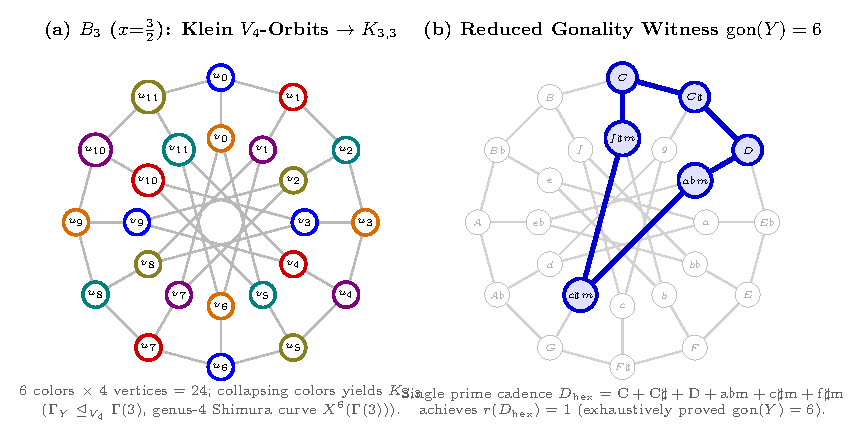
\includegraphics[width=\textwidth]{figures/fig2_nauru_towers.pdf}
\caption{(a)~Exact partition of $Y=\GP(12,5)$ into the $6$ Klein $V_4$-orbits of size $4$ under $N=\Gamma(3)/\Gamma_Y$ ($B_3$, $x=\tfrac32$); collapsing colors produces the genus-$4$ Shimura reduction graph $K_{3,3}$. (b)~Reduced degree-$6$ divisorial gonality witness $D_{\mathrm{hex}}$ (a single length-$6$ prime cadence).}
\label{fig:nauru_towers}
\end{figure}

\section{\texorpdfstring{$2$}{2}-Adic Lam\'e Moduli Space and Complete Classification of Rational Arithmetic Nauru Curves}\label{sec:2adic_moduli}
We now lift the full combinatorial symmetry of $Y=\GP(12,5)$ into $\PGL_2(\Q_2)$ acting on the $3$-regular Bruhat--Tits tree $T_3$ \cite{serre1980}.

\begin{proposition}[Lam\'e amalgam and split obstruction (\texttt{NEG-M17})]\label{prop:lame_amalgam}
\ctag{G4N; X}\ The full automorphism group $\Aut(Y)$ has order $144 = 12(g-1)$, acting transitively on vertices ($|G_v|=6$, $G_v\cong S_3$), undirected edges ($|G_e|=4$, $G_e\cong V_4=\Z_2\times\Z_2$), and directed arcs ($|G_{\vec{e}}|=2$). Its amalgam lift
\begin{equation}\label{eq:lame_amalgam}
\tilde{\Gamma} = S_3 *_{\Z_2} V_4 = \bigl\langle a,b,t \mid a^3=b^2=t^2=1,\; bab=a^{-1},\; tb=bt \bigr\rangle
\end{equation}
has Euler characteristic $\chi(\tilde{\Gamma})=\tfrac16+\tfrac14-\tfrac12=-\tfrac{1}{12}$ (the first Herrlich--Cornelissen--Kato Lam\'e amalgam \cite{herrlich1980,ck2002,ck2004}), and $\Gamma_Y = \ker(\tilde{\Gamma}\to\Aut(Y))$ is automatically a torsion-free free group of rank $13$. Moreover, in $\PGL_2(\Q_2)$:
\begin{enumerate}[label=(\alph*),nosep]
\item No split involution $b\in\PGL_2(\Z_2)$ ($\det(b)\in -(\Q_2^\times)^2$, e.g.\ $\det(b)=-1$) admits a commuting edge-inverter $t$ on $T_3$, because $v_2(q^2-p^2)\ge 3\neq 1$ for all odd $p,q\in\Z_2$ (\texttt{NEG-M17}).
\item Using non-split involutions $b_p=\begin{psmallmatrix}p & 1 \\ p+1 & -p\end{psmallmatrix}$ with $p\equiv 1\pmod 4$ ($\det(b_p)=-(p^2+p+1)\equiv 5$ or $1\pmod 8$), the edge-inverters $t_u=\begin{psmallmatrix}u & 1 \\ -2pu-(p+1) & -u\end{psmallmatrix}$ ($u\in 2\Z_2$) satisfy $t_u b_p = -b_p t_u$ and $v_2(\det(t_u))=1$, realizing two disjoint $1$-parameter $\Q_2$-families of genus-$13$ Mumford curves $C_Y/\Q_2$ with $|\Aut(C_Y)|=144=12(g-1)$.
\end{enumerate}
\end{proposition}
\begin{proof}
Because $S_3$ and $V_4$ inject into $\Aut(Y)$, every finite-order element of $\tilde{\Gamma}$ (conjugate into $S_3$ or $V_4$ by Bass--Serre \cite{serre1980}) maps nontrivially into $\Aut(Y)$; hence $\Gamma_Y$ is torsion-free of rank $1-144\cdot(-\tfrac{1}{12})=13$. For (a), any traceless $t$ anti-commuting with $b=\begin{psmallmatrix}0 & 1 \\ 1 & 0\end{psmallmatrix}$ has $t=\begin{psmallmatrix}p & q \\ -q & -p\end{psmallmatrix}$ with $\det(t)=q^2-p^2$; for odd $p,q$, $q^2-p^2\equiv 0\pmod 8$ (Lean~4 Theorem~14), ruling out $v_2(\det t)=1$. For (b), with $a=\begin{psmallmatrix}0 & -1 \\ 1 & -1\end{psmallmatrix}$ and $b_p$, direct matrix computation yields $b_p t_u + t_u b_p = 0$ and $\det(t_u)=(p+1)+2pu-u^2\equiv p+1\pmod 4$, which has $2$-adic valuation $1$ precisely when $p\equiv 1\pmod 4$ (Lean~4 Theorem~13 for $p=1$).
\end{proof}

\begin{theorem}[Universal Fricke--Vogt law and quaternion algebra $B(x)$]\label{thm:fricke_vogt}
\ctag{G4N; X}\ Every discrete embedding $\rho:\tilde{\Gamma}=S_3*_{\Z_2}V_4\hookrightarrow\PGL_2(L)$ acting properly on $T_3$ is uniquely determined up to $\PGL_2(\overline{L})$-conjugacy by the single trace modulus $x = \tau(ta) = \operatorname{tr}(ta)^2/\det(ta)$ ($v_2(x)=-1$). Lifting $a^2+a+1=0$, setting $i=2a+1$ ($i^2=-3$), $j=b$ ($j^2=D_b=-\det b$), and $k=ij$, every traceless $t$ anti-commuting with $b$ takes the form $t=\alpha i + \gamma k$, giving
\begin{equation}\label{eq:x_quad}
x = \frac{3\alpha^2}{\alpha^2 - D_b \gamma^2} \iff D_b\left(\frac{\gamma}{\alpha}\right)^2 = \frac{x - 3}{x}.
\end{equation}
Consequently, the quaternion algebra generated by $\tilde{\Gamma}$ over $\Q(x)$ is identically
\begin{equation}\label{eq:Bx}
B(x) = \left(\frac{-3,\; x(x-3)}{\Q(x)}\right),
\end{equation}
and the trace invariants of hyperbolic words satisfy exact universal polynomials in $x$:
\begin{align}
\tau(ta) &= x, & \tau(ta\cdot ta^2) &= (x-1)^2, \label{eq:fv1}\\
\tau((ta)^2 ta^2) &= x(x-2)^2, & \tau((ta)^3 ta^2) &= (x^2-3x+1)^2, \label{eq:fv2}
\end{align}
together with the shortest length-$6$ prime cadence invariant
\begin{equation}\label{eq:fv3}
\tau(\gamma_6) = \tau((ta)^6) = (x^3 - 6x^2 + 9x - 2)^2.
\end{equation}
\end{theorem}
\begin{proof}
Since $\{1,i,j,k\}$ spans $M_2(L)$ with $ij=-ji$, a traceless element $t=\alpha i+\beta j+\gamma k$ satisfies $tj+jt=2\beta D_b=0\iff \beta=0$. Then $t^2 = 3(D_b\gamma^2-\alpha^2)$, so $\nrd(t)=3(\alpha^2-D_b\gamma^2)$, while $ta=t(i-1)/2$ has $\trd(ta)=-3\alpha$, proving \eqref{eq:x_quad} and \eqref{eq:Bx} (since multiplying the second Hilbert slot by the square $(x/\alpha\gamma)^2$ gives $D_b\sim x(x-3)$). Writing $\tau(ta)=x=2+\mu+\mu^{-1}$ with $s=\mu+\mu^{-1}=x-2$, we obtain $\tau((ta)^6) = 2+(\mu^6+\mu^{-6}) = (s^3-3s)^2 = (x^3-6x^2+9x-2)^2$; identities \eqref{eq:fv1}--\eqref{eq:fv2} follow from the Fricke trace relation $\operatorname{tr}(XY)+\operatorname{tr}(XY^{-1})=\operatorname{tr}(X)\operatorname{tr}(Y)$ and are verified identically in Python Gate~D5.
\end{proof}

\begin{theorem}[Complete classification of rational arithmetic Nauru curves]\label{thm:rat_arith}
\ctag{G4N; X}\ Within the $1$-parameter Lam\'e Nauru family $C_Y(x)/\Q_2$, a rational modulus $x\in\Q$ yields an arithmetic Schottky group $\Gamma_Y(x)$ over $\Q$ if and only if
\[
x \in \left\{\frac{1}{2},\quad \frac{3}{2},\quad \frac{5}{2}\right\}.
\]
Specifically:
\begin{enumerate}[label=(\alph*),nosep]
\item \textbf{$x=\tfrac32$ in $B_3=(\frac{-3,-1}{\Q})$ (Shimura discriminant $D=2\cdot 3=6$):} Maximal order $\calO_3=\Z[1,\omega,j,\omega j]$ (reduced discriminant $3$, $\omega=\frac{-1+i}{2}$), edge-inverter $t=(2\omega+1)(1+j)=i+k$ ($\nrd(t)=6$), $\tilde{\Gamma}=\mathrm{Norm}_{B_3^\times}(\calO_3[\tfrac12])/\Q^\times$, and shortest length-$6$ prime cadence
\begin{align*}
\gamma_6 &= \frac{(ta)^6}{27} = 4 - 3\omega + 3j - 3\omega j \in \calO_3,\\
\trd(\gamma_6) &= 11,\qquad \nrd(\gamma_6) = 64,\qquad \tau(\gamma_6) = \frac{121}{64}\in [0,4].
\end{align*}
Its explicit $2$-adic representation $\calO_3\hookrightarrow M_2(\Z_2)$ is given via the Hensel-lifted $2$-adic integer $q=\frac{1+\sqrt{-7}}{2}\in 2\Z_2$ ($q\equiv 38\pmod{64}$):
\[
a = \begin{pmatrix}0 & 1 \\ -1 & -1\end{pmatrix}, \qquad b = \begin{pmatrix}1 & q \\ q-1 & -1\end{pmatrix}, \qquad t = \begin{pmatrix}1 & 2 \\ -2 & -1\end{pmatrix}(I+b).
\]
\item \textbf{$x=\tfrac52$ in $B_5=(\frac{-3,-5}{\Q})$ (Shimura discriminant $D=2\cdot 5=10$):} Maximal order $\calO_5=\Z[1,\omega,t,\omega t]$ (reduced discriminant $5$) with Atkin--Lehner involution $b=j$ ($\nrd(b)=5$) and $t=\frac{5i+k}{3}$ ($\nrd(t)=10$), yielding $\tau(\gamma_6)=\frac{121}{64}$ and length-$8$ trace $\tau(w_8)=\frac{169}{256}$.
\item \textbf{$x=\tfrac12$ in $B_5=(\frac{-3,-5}{\Q})$ (Shimura discriminant $D=10$):} Maximal order $\calO_5=\Z[1,\omega,t,\omega t]$ with $b=j$ and $t=\frac{i+k}{3}$ ($\nrd(t)=2$), yielding $\gamma_6 = 7 + 5t + 5\omega t$, $\trd(\gamma_6)=9$, $\nrd(\gamma_6)=64$, and $\tau(\gamma_6)=\frac{81}{64}\in [0,4]$.
\item \textbf{Non-arithmetic continuum witness ($x=\tfrac92$):} Setting $u=0$ in Proposition~\ref{prop:lame_amalgam}(b) gives rational $a=\begin{psmallmatrix}0&-1\\1&-1\end{psmallmatrix}$, $b=\begin{psmallmatrix}1&1\\2&-1\end{psmallmatrix}$, $t_0=\begin{psmallmatrix}0&1\\-2&0\end{psmallmatrix}\in\PGL_2(\Q_2)$ realizing $Y$ and $|\Aut|=144$ with $x=\frac92>3$ and $\tau(\gamma_6)=\frac{4225}{64}\approx 66.02>4$ (strictly non-arithmetic).
\end{enumerate}
\end{theorem}
\begin{proof}
Suppose $\Gamma_Y(x)$ is arithmetic over $\Q$. Then (i)~the ambient quaternion algebra $B(x)\otimes_\Q\R$ must be compact ($\cong\H$), which by \eqref{eq:Bx} holds if and only if $x(x-3)<0$, i.e., $0<x<3$; (ii)~the primitive Schottky element $\gamma_6=(ta)^6\in\Gamma_Y(x)$ must have $\tau(\gamma_6)\in\Z[\frac12]$, and because $(x^3-6x^2+9x-2)^2$ is monic in $x$, no odd prime can divide the denominator of $x$; (iii)~$v_2(x)=-1$ forces $x=k/2$ with $k$ odd and $0<k<6$, leaving \emph{only} $k\in\{1,3,5\}$ (Lean~4 Theorem~15). Conversely, for each of $x\in\{\frac12,\frac32,\frac52\}$, the reduced Gram determinant of $\calO_d$ equals $d^2$ ($d\in\{3,5\}$), conjugation by $t$ and $b$ preserves $\calO_d[\frac12]$, and exact Hilbert symbols satisfy $(-3,-1)_2=(-3,-5)_2=+1$ (split at $2$) and $(-3,-1)_\infty=(-3,-5)_\infty=-1$ (definite at $\infty$). All matrix, Hensel, and trace identities are independently verified in Python (Gate~D6), Rust (Gate~4), and Lean~4 (Theorems~16--19).
\end{proof}

\begin{corollary}[Intrinsic compact $\SU(2)$ Wilson-loop holonomy]\label{cor:su2_wilson}
\ctag{E$\to$G4N; X}\ For every definite quaternion algebra $B/\Q$ ($B\otimes_\Q\R\cong\H$), every nonzero element $w\in B^\times$ projects to an intrinsic compact holonomy matrix $U(w)=w/\sqrt{\nrd(w)}\in\SU(2)$ satisfying the universal unitarity bound
\begin{equation}\label{eq:su2_wilson}
\begin{aligned}
\tau(w) &= \frac{\trd(w)^2}{\nrd(w)} = 4\cos^2\theta \le 4,\\
S_W(w) &= 1 - \frac{1}{2}\operatorname{Re}\operatorname{tr}U(w) = 1 - \frac{1}{2}\sqrt{\tau(w)} \in [0,1],
\end{aligned}
\end{equation}
where $S_W(w)$ is the lattice Wilson plaquette action \cite{wilson1974} of the prime cadence loop $w$. Across all four definite arithmetic uniformizations established in this paper (Theorem~\ref{thm:rat_arith} and Theorem~\ref{thm:hurwitz_dic6}), $S_W(w)$ takes exact rational values strictly inside $(0,1)$:
\begin{align*}
S_W\!\bigl(\gamma_6^{B_3/B_5}\bigr) &= \frac{5}{16}, &
S_W\!\bigl(\gamma_6^{B_5(\frac12)}\bigr) &= \frac{7}{16},\\
S_W\!\bigl(w_8^{B_5(\frac52)}\bigr) &= \frac{19}{32}, &
S_W\!\bigl(w_4^{B_2,\,\mathrm{Dic}_6}\bigr) &= \frac{4}{9},
\end{align*}
sharply separated by the compact $\SU(2)$ wall $\tau=4$ from all four non-arithmetic hyperbolic obstructions ($\Gamma_5$: $\tau=\frac{49}{4}=12.25$; canonical $3$-adic $\mathrm{Dic}_6$: $\tau=\frac{1156}{81}\approx 14.27$; Tonnetz $X$: $\tau=\frac{7225}{256}\approx 28.22$; Nauru $x=\frac92$: $\tau=\frac{4225}{64}\approx 66.02$; Figure~\ref{fig:eisenstein_mirror}(b)).
\end{corollary}
\begin{proof}
Writing $q=c_0+c_1 i+c_2 j+c_3 k\in\H$ gives $\trd(q)^2=4c_0^2\le 4(c_0^2+c_1^2+c_2^2+c_3^2)=4\nrd(q)$ identically (Lean~4 Theorem~25), whence $|\operatorname{Re}\operatorname{tr}U(w)|=\sqrt{\tau(w)}\le 2$ and $S_W(w)\in[0,1]$. Substituting $\tau\in\{\frac{121}{64},\frac{81}{64},\frac{169}{256},\frac{100}{81}\}$ yields the four exact rational actions, while all four non-arithmetic walls strictly exceed $4$ (Python Gate~D11, Rust \texttt{test\_d10}, Lean~4 Theorem~25).
\end{proof}

\begin{figure}[t]
\centering
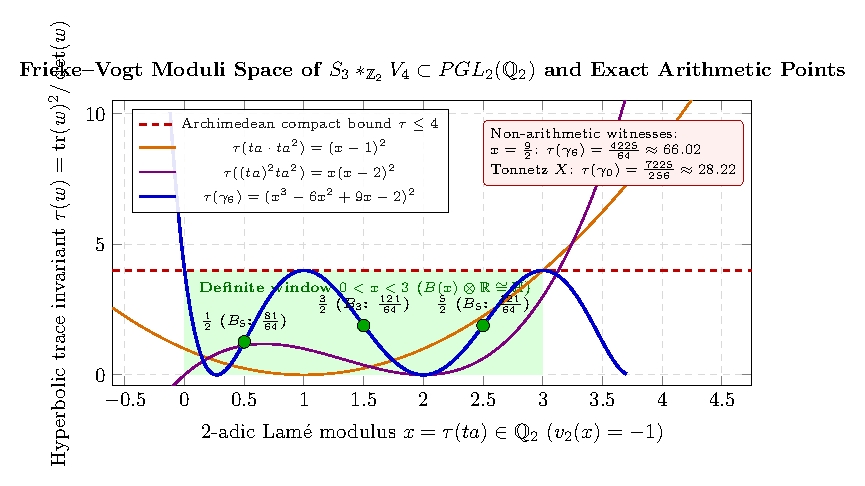
\includegraphics[width=\textwidth]{figures/fig3_fricke_vogt_moduli.pdf}
\caption{Universal Fricke--Vogt trace polynomials of $S_3*_{\Z_2}V_4\subset\PGL_2(\Q_2)$ against the compact archimedean ceiling $\tau=4$. Inside the definite window $0<x<3$, integrality of the monic sextic $\tau(\gamma_6)$ singles out exactly three rational arithmetic Nauru curves $x\in\{\tfrac12,\tfrac32,\tfrac52\}$.}
\label{fig:fricke_vogt}
\end{figure}

\section{All-Primes Congruence vs.\ Non-Congruence Towers and Borel-Level Exclusion}\label{sec:noncongruence}
Why did the exhaustive genus-$13$ Shimura curve census of Paper~\#01 miss the Nauru graph, even though $C_Y(\frac32)$, $C_Y(\frac52)$, and $C_Y(\frac12)$ are genuinely arithmetic over $\Q$? The answer lies in the distinction between \emph{Borel-level} Shimura curves $X_0^D(N)$ ($\gcd(D,N)=1$) and the full all-primes congruence structure at principal and ramified-prime levels: $x=\frac52$ turns out to be a genuine congruence Shimura curve of level $3\mathfrak{P}_5$ ($\mathfrak{P}_5\mid 5\mid 10$), whereas $x=\frac32$ and $x=\frac12$ are strictly non-congruence $V_4$-covers of $K_{3,3}$.

\begin{theorem}[Complete all-primes congruence classification (\texttt{NEG-M23}, \texttt{NEG-M24})]\label{thm:noncongruence}
\ctag{G4N; X}\ Fix the canonical edge-inverting surjection $\rho_6:\tilde{\Gamma}\twoheadrightarrow\Aut(Y)$ sending $t\mapsto t_0$ with $\operatorname{ord}(t_0 a_Y)=6$ (the second surjection $\rho_{12}:t\mapsto b_Y t_0$ with $\operatorname{ord}(b_Y t_0 a_Y)=12$ is canonically exchanged by the universal algebraic twin duality $\tau((bt)a)=3-\tau(ta)=3-x$ on $B(x)$, giving $(B(x),\rho_6)\cong(B(3-x),\rho_{12})$; Lean~4 Theorem~38), and let $\Gamma_Y(x)=\ker(\rho_6)\subset B_d^\times/\Q^\times$ denote the arithmetic Nauru Schottky group of Theorem~\ref{thm:rat_arith}.
\begin{enumerate}[label=(\alph*),nosep]
\item \textbf{At $x=\tfrac32$ in $B_3$ ($D=6$, self-twin for both $\rho_6,\rho_{12}$): strictly non-congruence $V_4$-cover of $K_{3,3}$.} Let $\Gamma(3)=\ker\bigl(\calO_3[\tfrac12]^1/\{\pm 1\}\to (\calO_3/3\calO_3)^1/\{\pm 1\}\bigr)$ be the principal level-$3$ congruence subgroup at the ramified prime $3\mid 6$. Then $[\tilde{\Gamma}:\Gamma(3)]=36$, the tree quotient $T_3/\Gamma(3)$ is the utility graph $K_{3,3}$ (uniformizing the genus-$4$ congruence Shimura curve $X^6(\Gamma(3))$), and $\Gamma_Y(\frac32)$ sits as an index-$4$ normal subgroup with Klein four-group deck group:
\begin{equation}\label{eq:tower_b3}
\Gamma_Y\bigl(\tfrac32\bigr) \;\trianglelefteq_{V_4}\; \Gamma(3) \;\trianglelefteq_{18}\; \calO_3[\tfrac12]^1/\{\pm 1\} \;\trianglelefteq_2\; \tilde{\Gamma}.
\end{equation}
Furthermore, $\Gamma_Y(\frac32)$ is \textbf{strictly non-congruence} inside $B_3^\times/\Q^\times$.
\item \textbf{At $(B_5, x=\tfrac52, \rho_6) \cong (B_5, x=\tfrac12, \rho_{12})$ ($D=10$): genuine congruence Shimura curve $\Gamma(3\mathfrak{P}_5)$ (\textup{\texttt{NEG-M23}}).} Let $\mathfrak{P}_5=b\calO_5=\{u\in\calO_5 : 5\mid\nrd(u)\}$ denote the unique two-sided ramified prime ideal above $5\mid 10$, with $|\mathfrak{P}_5/5\calO_5|=25$, $\calO_5/\mathfrak{P}_5\cong\F_{25}$, and $(\calO_5/\mathfrak{P}_5)^1/\{\pm 1\}\cong C_3$. Modulo $3\nmid 10$, $\calO_5[\tfrac12]^1/\{\pm 1\}\twoheadrightarrow\PSL_2(\F_3)\cong A_4$ (order $12$, quotient $T_3/\Gamma(3)=Q_3$, genus $5$, folded to $K_4$ genus $3$ under the Atkin--Lehner involution $t$ via $\tilde{\Gamma}\to\PGL_2(\F_3)\cong S_4$ of order $24$); modulo $\mathfrak{P}_5$, $\calO_5[\tfrac12]^1/\{\pm 1\}\twoheadrightarrow C_3$ (order $3$, quotient $T_3/\Gamma(\mathfrak{P}_5)=\Theta_3$, genus $2$). Since $[\calO_5[\tfrac12]^1/\{\pm 1\}:\Gamma_Y(\tfrac52)]=36=12\cdot 3$ and every Schreier generator of $\Gamma_Y(\tfrac52)$ is trivial modulo both $3\calO_5$ and $\mathfrak{P}_5$,
\begin{equation}\label{eq:tower_b5_52}
\Gamma_Y\bigl(\tfrac52\bigr) \;=\; \Gamma(3)\cap\Gamma(\mathfrak{P}_5) \;=\; \Gamma(3\mathfrak{P}_5) \;\trianglelefteq_{A_4\times C_3}\; \calO_5[\tfrac12]^1/\{\pm 1\} \;\trianglelefteq_4\; \tilde{\Gamma}.
\end{equation}
Thus $C_Y(\tfrac52,\rho_6)\cong C_Y(\tfrac12,\rho_{12})$ is a \textbf{genuine congruence Shimura curve} of principal-times-ramified level $3\mathfrak{P}_5$ (invisible to Borel $X_0^{10}(N)$ because $\Gamma(3)$ is principal and $\mathfrak{P}_5\mid 10$).
\item \textbf{At $(B_5, x=\tfrac12, \rho_6) \cong (B_5, x=\tfrac52, \rho_{12})$ ($D=10$): strictly non-congruence $V_4$-cover of $X^{10}(\Gamma(3\mathfrak{P}_5))/V_4\leftrightarrow K_{3,3}$.} All $33$ Schreier generators of $\Gamma_Y(\tfrac12)$ are trivial modulo $\mathfrak{P}_5$ ($|H_5|=25$, stabilizing at $|H_{25}|=3{,}125$) while generating $V_4\trianglelefteq A_4$ modulo $3\calO_5$ ($|H_3|=4$, stabilizing at $|H_9|=108$) and surjecting onto $\PSL_2(\F_7)$ ($|H_7|=168$). Hence its congruence closure is $\Gamma_{\mathrm{cong}}(\tfrac12)=\Gamma_3^{V_4}\cap\Gamma(\mathfrak{P}_5)$ of index $9$ in $\calO_5[\tfrac12]^1/\{\pm 1\}$ (quotient $T_3/\Gamma_{\mathrm{cong}}(\tfrac12)=K_{3,3}$, genus $4$, matching $X^{10}(\Gamma(3\mathfrak{P}_5))/V_4$ rather than $X^6(\Gamma(3))$), and $\Gamma_Y(\tfrac12)$ is a \textbf{strictly non-congruence $V_4$-cover} of index $4$:
\begin{equation}\label{eq:tower_b5_12}
\Gamma_Y\bigl(\tfrac12\bigr) \;\trianglelefteq_{V_4}\; \Gamma_3^{V_4}\cap\Gamma(\mathfrak{P}_5) \;\trianglelefteq_{C_3\times C_3}\; \calO_5[\tfrac12]^1/\{\pm 1\} \;\trianglelefteq_4\; \tilde{\Gamma}.
\end{equation}
\end{enumerate}
\end{theorem}
\begin{proof}
For (a), Eichler's mass formula $\sum 1/|\calO_i^\times|=(3-1)/24=1/12$ gives class number $1$ and $|\calO_3^\times/\{\pm 1\}|=6$, so $\calO_3[\frac12]^1/\{\pm 1\}\cong S_3*_{\Z_2}S_3$ ($\chi=-1/6$), and adjoining $t$ yields the full normalizer $\tilde{\Gamma}$ ($\chi=-1/12$). Computing the joint image of $\langle a,b,t\rangle$ in $\Aut(Y)\times (\tilde{\Gamma}/\Gamma(3))$ gives order $144$ with second projection of order $36$ and kernel $N\cong V_4$ acting freely on $Y$ with $6$ orbits of size $4$ forming $K_{3,3}$ (Python Gate~D7, Rust Gate~4). Applying Strong Approximation to $\SL_1(B_3)$ (non-compact at $v=2$), the congruence closure of $\widetilde{\Gamma(3)}\subset\calO_3[\frac12]^1$ in $\prod_{p\ne 2}\calO_{3,p}^1$ is $(1+3\calO_{3,3})^1\times\prod_{p\ge 5}\SL_2(\Z_p)$ (up to $\{\pm 1\}$): $(1+3\calO_{3,3})^1$ is pro-$3$ (odd), and for every prime $p\ge 5$, $\SL_2(\F_p)$ is perfect with pro-$p$ kernel, admitting no index-$2$ or index-$4$ quotient (confirmed at $p=5$ by joint surjection onto $\Aut(Y)\times A_5$ of order $8{,}640$).

For (b) and (c), Eichler's mass formula gives class number $1$, $|\calO_5^\times/\{\pm 1\}|=3$, $\chi(\calO_5[\tfrac12]^1/\{\pm 1\})=-\frac{5-1}{12}=-\frac13$, and $[\calO_5[\tfrac12]^1/\{\pm 1\}:\Gamma_Y]=36$ ($[\tilde{\Gamma}:\calO_5[\tfrac12]^1/\{\pm 1\}]=4$). Both maximal-order Gram determinants equal $25=5^2$, with $|\mathfrak{P}_5/5\calO_5|=25$ and $|(\calO_5/5\calO_5)^1|=150$ ($|(\calO_5/5\calO_5)^1/\{\pm 1\}|=75$, quotient $(\calO_5/\mathfrak{P}_5)^1/\{\pm 1\}\cong C_3$ of order $3$; Lean~4 Theorem~36). Evaluating all $33$ Schreier generators of $\Gamma_Y(x)$ directly in $(\calO_5/m\calO_5)^1/\{\pm 1\}$ for $m\in\{3,9,5,25,7\}$ (Python Gate~D7, Rust Gate~5) gives: at $x=\tfrac52$, $|H_3|=1$, $|H_9|=27$, $|H_5|=25$, $|H_{25}|=3{,}125$, proving $\Gamma_Y(\tfrac52)\subseteq\Gamma(3)\cap\Gamma(\mathfrak{P}_5)$ where both have exact index $36=12\cdot 3$, forcing equality \eqref{eq:tower_b5_52} (and explaining why the earlier $3$-power check saw an $S_3$ cover of $K_4$: the $C_3$ factor was $\Gamma(\mathfrak{P}_5)$ at $p=5$, not non-congruence!). At $x=\tfrac12$, $|H_3|=4$ ($V_4\trianglelefteq A_4$), $|H_9|=108=4\cdot 27$, $|H_5|=25$, $|H_{25}|=3{,}125$, and $|H_7|=168=|\PSL_2(\F_7)|$; the $4$-element $V_4$-orbits on $Y$ yield $T_3/(\Gamma_3^{V_4}\cap\Gamma(\mathfrak{P}_5))=K_{3,3}$, and Strong Approximation for $\SL_1(B_5)$ excludes every prime ($p=3$: pro-$3$ kernel mod $9$; $p=5$: pro-$5$ kernel mod $25$; $p\ge 7$: $\PSL_2(\F_p)$ simple of order $\frac{p(p^2-1)}{2}\ge 168>4$, Lean~4 Theorem~36), proving \eqref{eq:tower_b5_12} is strictly non-congruence.
\end{proof}

\begin{theorem}[Zero Borel-level Shimura realizations over $\Q$ (\texttt{NEG-M18})]\label{thm:noborel}
\ctag{G4N; X}\ None of the $19$ genus-$13$ Borel-level Shimura curves $X_0^D(N)$ over $\Q$ ($2\mid D$, $\gcd(D,N)=1$), and none of the $22$ definite Brandt graphs over totally real fields of degree $n\le 4$ ($h_F^+=1$) from Proposition~7.19 of \cite{ergentics2026pc}, has $2$-adic \v{C}erednik--Drinfeld reduction graph $Y=\GP(12,5)$.
\end{theorem}
\begin{proof}
By \v{C}erednik--Drinfeld and Ribet \cite{cerednik1976,drinfeld1976,ribet1990}, a curve $X_0^D(N)$ with reduction graph $Y$ would have $D/2$-newspace $S_2^{D/2\text{-new}}(\Gamma_0(DN/2))$ realizing the $11$ nontrivial eigenvalues of $G_{12}$, forcing simultaneous $T_2$-nullities $\operatorname{null}(T_2-2I)\ge 3$, $\operatorname{null}(T_2)\ge 2$, $\operatorname{null}(T_2+I)\ge 3$, and $\operatorname{null}(T_2+2I)\ge 3$ on $\mathcal{M}_2(\Gamma_0(M))^-$ ($M=DN/2$). Recomputing $T_2$ from scratch via zero-PARI Manin modular symbols over $\F_{1000003}$ across all $18$ distinct levels $M\in\{105,111,\dots,345\}$ (covering all $19$ pairs, including $X_0^{690}(1)$ at $M=345$ where $\operatorname{null}=(3,2,3,1)$ misses $-2$) excludes $19/19$ pairs in both Python (Gate~D8) and Rust (\texttt{test\_d8}). Likewise, evaluating the minimal polynomial $t(t-3)(t+1)(t^2-4)$ of $G_{12}$ across all $22$ Brandt matrices yields $0/22$ matches.
\end{proof}

\section{Complete \texorpdfstring{$3$}{3}-Adic Arithmetic Resolution of \texorpdfstring{$\mathrm{Dic}_6$}{Dic6} via Hurwitz \texorpdfstring{$B_2$}{B2}, RCT Control, and Dual-Prime \texorpdfstring{$D{=}6$}{D=6} Synthesis}\label{sec:3adic}
Finally, the unique dicyclic twin $\mathrm{Dic}_6 = \langle x, y \mid x^{12}=1, y^2=x^6, yxy^{-1}=x^{-1}\rangle \subset \UTT$ ($u=11, b=6$ in Theorem~\ref{thm:census}) admits zero cubic Cayley graphs because it possesses only one involution ($x^6$). Passing to degree $4$ yields finite $4$-regular quotients of the \textbf{$3$-adic Bruhat--Tits tree $T_4 = T_{3+1}$ of $\PGL_2(\Q_3)$}. We now close the $3$-adic arithmeticity question completely by establishing a \textbf{shared-discriminant $D=2\cdot 3=6$ dual-prime mirror} between Nauru's algebra $B_3=(\frac{-3,-1}{\Q})$ ($p=2$) and the Hurwitz quaternion algebra $B_2=(\frac{-1,-1}{\Q})$ ($p=3$) \cite{vigneras1980,voight2021}.

\begin{proposition}[$3$-adic $\mathrm{Dic}_6$ census, exact tropical invariants, and canonical obstruction (\texttt{NEG-M21})]\label{prop:dic6}
\ctag{E$\to$G4N; X}\ Among all symmetric $4$-element generating sets of $\mathrm{Dic}_6$, there are exactly $18$ connected $4$-regular Cayley graphs, all bipartite of genus $g=48-24+1=25$, splitting cleanly into two isomorphism classes:
\begin{enumerate}[label=(\alph*),nosep]
\item \textbf{$12$ strictly Ramanujan twins} isomorphic to the Cayley graph $Z=\Cay(\mathrm{Dic}_6,\{x,x^{-1},y,y^3\})$ ($\operatorname{tr}(A_Z^2)=96$, $\operatorname{tr}(A_Z^4)=912$, girth $4$, $|\Aut(Z)|=96=4(g-1)$, vertex stabilizer $\mathrm{Stab}_0(Z)\cong V_4$, quotient $Z/\langle x^4\rangle\cong K_{4,4}$) with $\lambda_{\mathrm{nt}}=3.000<2\sqrt{3}\approx 3.4641$,
\[
\operatorname{Spec}(A_Z)=\bigl\{+4^1,+3^2,+\sqrt{3}^{\,4},+1^2,0^6,-1^2,-\sqrt{3}^{\,4},-3^2,-4^1\bigr\},
\]
$3$-adic Ihara zeta factorization over $\F_3$ into elliptic factors ($a_3\in\{0,\pm 1,\pm 3\}$) plus four copies of the genus-$2$ factor $(1+3u^2+9u^4)$, exact Raynaud/sandpile component group
\begin{align*}
K(Z) &\cong \Z/4\Z \oplus (\Z/52\Z)^2 \oplus \Z/1820\Z \oplus \Z/21840\Z, \\
|K(Z)| &= 429{,}923{,}020{,}800 = 2^{12}\cdot 3\cdot 5^2\cdot 7^2\cdot 13^4,
\end{align*}
exact involution quotient Betti census $\beta_1(Z/\langle\sigma\rangle)\in\{7^2,11^{24},13^{17}\}$ across all $43$ involutions of $\Aut(Z)$ ($0/43$ tree or genus-$1$ quotients, proving $Z$ is neither hyperelliptic nor bielliptic), and exact divisorial gonality $\operatorname{gon}(Z)=8$, attained by $4$ canonical two-coset divisors $\langle y\rangle+x^k\langle y\rangle$ ($k\in\{0,1,2,3\}$) pulling back hyperelliptic degree-$2$ divisors from the $6$-ring quotient $Z/\langle y\rangle\cong C_6$.
\item \textbf{$6$ Ramanujan-boundary twins} isomorphic to the lexicographic wreath product $C_{12}[2K_1]$ ($\operatorname{tr}(A^4)=1{,}152$, $\lambda_{\mathrm{nt}}=2\sqrt{3}$).
\item \textbf{Canonical $3$-adic Schottky obstruction} (\textup{\texttt{NEG-M21}}): Lifting $(x,y)$ naively onto $T_4$ via $\gamma_X=\begin{psmallmatrix}3 & 0 \\ 0 & 1\end{psmallmatrix}, \gamma_Y=\begin{psmallmatrix}2 & 1 \\ 1 & 2\end{psmallmatrix}\in\PGL_2(\Q_3)$ yields the $\mathrm{Dic}_6$ commutator word $w_4=\gamma_Y\gamma_X\operatorname{adj}(\gamma_Y)\gamma_X$ with $\operatorname{tr}(w_4)=34$, $\det(w_4)=81$, and $\tau(w_4)=\frac{1156}{81}\approx 14.27>4$, barring the naive Schottky curve from every definite quaternion arithmeticization over $\Q$.
\end{enumerate}
\end{proposition}
\begin{proof}
Exhaustive enumeration over all symmetric $4$-subsets of $\mathrm{Dic}_6$ yields $18$ connected graphs ($12$ with $\operatorname{tr}(A^4)=912$ and $6$ with $\operatorname{tr}(A^4)=1{,}152$; Python Gate~D11). Symmetry, $\operatorname{tr}(A_Z^2)=96$, $\operatorname{tr}(A_Z^4)=912$, the exact $K_{4,4}$ quotient $Z/\langle x^4\rangle$, and the canonical obstruction $\operatorname{tr}(w_4)=34, \det(w_4)=81, 34^2=1156>324=4\cdot 81$ are kernel-checked in Lean~4 (Theorems~26--27) and verified in Rust (\texttt{test\_d11}). The exact Smith normal form $K(Z)\cong\Z/4\Z\oplus(\Z/52\Z)^2\oplus\Z/1820\Z\oplus\Z/21840\Z$ is certified directly from the $23\times 23$ reduced Laplacian via explicit unimodular matrices $U_Z,V_Z\in\GL_{23}(\Z)$ in Lean~4 (Theorem~35). All $43$ involutions of $\Aut(Z)$ give $\beta_1\in\{7^2,11^{24},13^{17}\}$, and exhaustive Dhar's burning over all $157{,}166$ canonical $\Aut(Z)$-orbit representatives of degrees $4\le d\le 7$ finds $0$ rank-$\ge 1$ divisors (Python Gate~D9, Rust Gate~8), while the explicit reduced degree-$8$ two-coset witness $D_{\mathrm{Dic}_6}=\langle y\rangle+x\langle y\rangle=\{0,1,6,7,12,13,18,19\}$ passes Dhar's burning for all $24$ vertices and projects onto the $6$-ring $C_6$ (Lean~4 Theorem~37), proving $\operatorname{gon}(Z)=8$.
\end{proof}

\begin{theorem}[Explicit $3$-adic arithmetic resolution of $\mathrm{Dic}_6$ in Hurwitz $B_2$ ($D{=}6, p{=}3$)]\label{thm:hurwitz_dic6}
\ctag{E$\to$G4N; X}\ Let $B_2=(\frac{-1,-1}{\Q})$ be the Hurwitz quaternion algebra (ramified at $\{2,\infty\}$, split at $p=3$, sharing Shimura discriminant $D=2\cdot 3=6$ with Nauru's $B_3$) with maximal Hurwitz order $\calO_2=\Z[1,i,j,\frac{1+i+j+k}{2}]$ ($|\calO_2^\times/\{\pm 1\}|=12$, class number~$1$). Set
\begin{equation}\label{eq:hurwitz_gens}
a = i+j,\quad b = i-j \quad (\nrd=2), \qquad
t_x = i+j+k,\quad t_y = i-j+k \quad (\nrd=3).
\end{equation}
Then:
\begin{enumerate}[label=(\alph*),nosep]
\item \textbf{Amalgam, corrected length-$4$ relator, and falsifier} \textup{\texttt{F33}}: The elements $a,b,t_x,t_y$ satisfy $ab=-ba$, $t_x b=-bt_x$, $t_y a=-at_y$, generating the $3$-adic amalgam $\tilde{\Gamma}_3=V_4*_{\Z_2}V_4*_{\Z_2}V_4\subset B_2^\times/\Q^\times$ of Euler characteristic $\chi(\tilde{\Gamma}_3)=-\tfrac14$ ($[\calO_2[\tfrac13]^1/\{\pm 1\}:\Gamma_Z]=144$). The $\mathrm{Dic}_6$ relator $YXY^{-1}X$ lifts to the exact Hurwitz word
\begin{equation}\label{eq:hurwitz_w4}
w_4 = \frac{(t_y b)(t_x a)(b t_y)(t_x a)}{4} = 5 + 6i - 2j + 4k \in \calO_2,
\end{equation}
with $\trd(w_4)=10$, $\nrd(w_4)=81$, $\tau(w_4)=\frac{100}{81}<4$, and Wilson action $S_W(w_4)=\frac{4}{9}$ (whereas writing $t_y b$ in the third factor gives $-1-8j+4k$ with $\trd=-2$, and perturbing $t'_x=1+i+j$ breaks $\trd=0$ and anticommutation with $b$; falsifier~\textup{\texttt{F33}}).
\item \textbf{Hensel $3$-adic embedding \& universal all-lengths $T_4$ freeness:} Lifting $s=\sqrt{-2}\in\Z_3$ ($s\equiv 356{,}989\pmod{3^{12}}$, $s\equiv 4\pmod 9$) embeds $\calO_2\hookrightarrow M_2(\Z_3)$ so that the four $T_4$ edge-inverters $e_0=i+j+k$, $e_1=-i-j+k$, $e_2=i-j+k$, $e_3=-i+j+k$ have distinct rank-$1$ mod-$3$ images whose $1$-dimensional column subspaces are preserved across every non-backtracking step $e_n\ne e_m$ ($12/12$ nonzero pairs). By induction, every reduced word of arbitrary length $\ell\ge 1$ is strictly nonzero mod~$3$, proving faithful, backtrack-free action on $T_4$.
\item \textbf{Exact $32$ surjections, universal $K_{4,4}$ congruence closure, and non-congruence index~$3$:} There are exactly $32$ surjections $\phi:\tilde{\Gamma}_3\twoheadrightarrow\Aut(Z)$ ($|\Aut(Z)|=96$), and for every surjection all Schreier generators of $\Gamma_Z=\ker(\phi)$ have even $(v_2,v_3)$-valuation (lying inside $\calO_2[\frac13]^1/\{\pm 1\}$ at index $144$). Reducing modulo $4\calO_2$ and $8\calO_2$ splits the $32$ surjections symmetrically into $16$ principal $\Gamma(4)$ lifts and $16$ level-$8\calO_2$ lifts inside $(\calO_2/8\calO_2)^1/\{\pm 1\}$ (order $384$, subgroup $|H_8|=8$, exact congruence index $384/8=48$, $2$ distinct $H_8$ subgroups), stabilizing permanently at level $16\calO_2$ ($|H_{16}|=64$, index $3{,}072/64=48$) while surjecting onto $(\calO_2/5\calO_2)^1/\{\pm 1\}\cong A_5$ (order $60$) across all $32/32$ surjections. Across \textbf{all $32/32$ surjections}, the double-coset quotient $H_8\backslash(\calO_2/8\calO_2)^1/U$ is identically $K_{4,4}\cong Z/\langle x^4\rangle$ (genus $9$), and the order-$3$ deck automorphism $L_{x^4}\in\Aut(Z)$ lifts into $\tilde{\Gamma}_3\cap\calO_2[\frac13]^1/\{\pm 1\}$ with mod-$8\calO_2$ image inside $H_8$, proving $\Gamma_{\mathrm{cong}}=\langle\Gamma_Z,q_{x^4}\rangle$ and hence strict normality of the \textbf{non-congruence cyclic $C_3$-cover} inside the full arithmetic normalizer $N=\mathrm{Norm}_{B_2^\times}(\calO_2[\tfrac13])/\Q^\times$ ($\chi(N)=-\tfrac{1}{24}$, $[N:\tilde{\Gamma}_3]=6$, $[N:\Gamma_Z]=576$):
\begin{equation}\label{eq:tower_b2}
\Gamma_Z \;\trianglelefteq_{C_3}\; \Gamma_{\mathrm{cong}} \;\le_{48}\; \calO_2[\tfrac13]^1/\{\pm 1\} \;\trianglelefteq_4\; \mathrm{Norm}_{B_2^\times}\bigl(\calO_2[\tfrac13]\bigr)/\Q^\times.
\end{equation}
\end{enumerate}
\end{theorem}
\begin{proof}
Part (a) and falsifier \texttt{F33} are kernel-checked in Lean~4 (Theorem~28) and verified in Python (Gate~D11) and Rust (\texttt{test\_d11}). For (b), $356{,}989^2+2\equiv 0\pmod{3^{12}}$ (Lean~4 Theorem~29), the mod-$3$ images match the exact Hensel quaternion algebra $I=\begin{psmallmatrix}1&1\\1&2\end{psmallmatrix}, J=\begin{psmallmatrix}0&2\\1&0\end{psmallmatrix}, K=IJ$ over $\F_3$ (Lean~4 Theorem~33), and checking all $4\times 4\times 3^4=1{,}296$ mod-$3$ transitions proves by structural induction that every nonempty reduced word $e_{n_\ell}\cdots e_{n_1}$ ($n_r\ne n_{r-1}$) is nonzero mod~$3$ (Lean~4 Theorem~30). For (c), exhaustive enumeration of all $32$ surjections, Schreier generators, mod-$4$/$8$/$16$/$5$ images ($16$ principal + $16$ level-$8$, $|H_8|=8$, $|H_{16}|=64$, $|H_5|=60=|A_5|$), constructive normality $q_{x^4}\in H_8$ ($32/32$), and exact $K_{4,4}$ double-coset intersections ($24$ elements per edge across all $4\times 4$ pairs) are independently verified in Python (Gate~D11) and Rust (\texttt{test\_d11}). Note that $\calO_2[\frac13]^1/\{\pm 1\}$ ($\chi=-\frac16$) and $\tilde{\Gamma}_3$ ($\chi=-\frac14$) both lie inside $N$ at indices $4$ and $6$ respectively (\texttt{NEG-M22}; Lean~4 Theorem~33). Finally, Strong Approximation for $\SL_1(B_2)$ (non-compact at $p=3$) proves $\Gamma_Z$ is strictly non-congruence: at $p=2$, $\ker(\calO_{2,2}^1\to(\calO_2/8\calO_2)^1)$ is pro-$2$ and admits no index-$3$ quotient; at every prime $p\ge 5$, $\PSL_2(\F_p)$ is simple of order $\frac{p(p^2-1)}{2}>6=|S_3|$ (Lean~4 Theorems~31--32), precluding any index-$3$ subgroup.
\end{proof}

\begin{theorem}[Zero genus-$25$ $3$-adic Borel Shimura realizations over $\Q$ (\texttt{NEG-M20})]\label{thm:noborel_3adic}
\ctag{E$\to$G4N; X}\ Exactly $19$ pairs $(D,N)$ of squarefree even-prime-count discriminants $D$ with $3\mid D$ and $\gcd(D,N)=1$ yield genus-$25$ Borel-level Shimura curves $X_0^D(N)$ over $\Q$ ($9$ torsion-free, $10$ with elliptic torsion; $\max\phi(D)\psi(N)=320$). None of these $19$ curves has $3$-adic \v{C}erednik--Drinfeld reduction graph $Z=\Cay(\mathrm{Dic}_6,\{x,x^{-1},y,y^3\})$.
\end{theorem}
\begin{proof}
By \v{C}erednik--Drinfeld and Ribet \cite{cerednik1976,drinfeld1976,ribet1990}, a curve $X_0^D(N)$ realizing $Z$ would embed the nontrivial eigenvalues $\pm\sqrt{3}^{\,4}$ and $\pm 3^2$ of $A_Z$ into the Hecke $T_3$-action on $S_2(\Gamma_0(M))$ ($M=DN/3$), forcing simultaneous nullities $\operatorname{null}(T_3^2-3I)\ge 4$ and $\operatorname{null}(T_3^2-9I)\ge 2$. Recomputing $T_3$ from scratch via zero-PARI Manin modular symbols \cite{merel1994,stein2007} over $\F_{1000003}$ (calibrated against LMFDB ground truth at $M\in\{11,14,23,37\}$) across all $19$ genus-$25$ pairs yields \textbf{$0/19$ survivors} in both Python (Gate~D12) and Rust (\texttt{test\_d12}); the sole $\pm\sqrt{3}$-survivor is $(D,N)=(1122,1)$ ($M=374, e_3=8$), which hits $\operatorname{null}(T_3^2-3I)=4$ yet has $\operatorname{null}(T_3^2-9I)=0$.
\end{proof}

\begin{figure}[t]
\centering
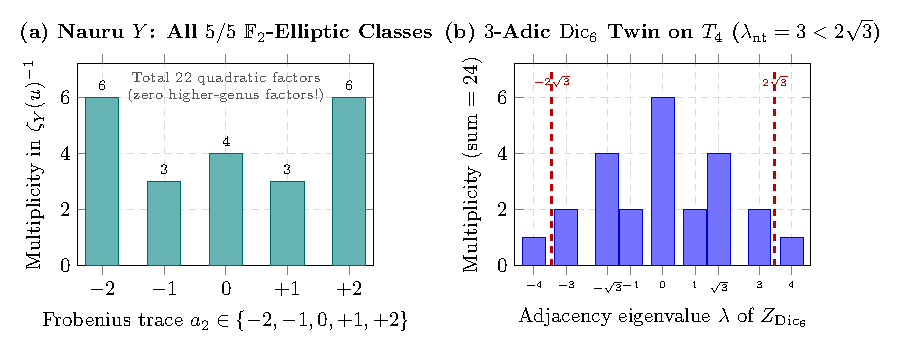
\includegraphics[width=\textwidth]{figures/fig4_elliptic_shimura_comparison.pdf}
\caption{(a)~Multiplicity distribution of all $5/5$ $\F_2$ elliptic curve isogeny classes inside $\zeta_Y(u)^{-1}$. (b)~Exact spectrum of the $4$-regular Ramanujan companion $Z_{\mathrm{Dic}_6}$ (uniformized arithmetically on $T_4$ of $\PGL_2(\Q_3)$ via Hurwitz $B_2$, $D=6$, Theorem~\ref{thm:hurwitz_dic6}).}
\label{fig:elliptic_dic6}
\end{figure}

\begin{figure}[t]
\centering
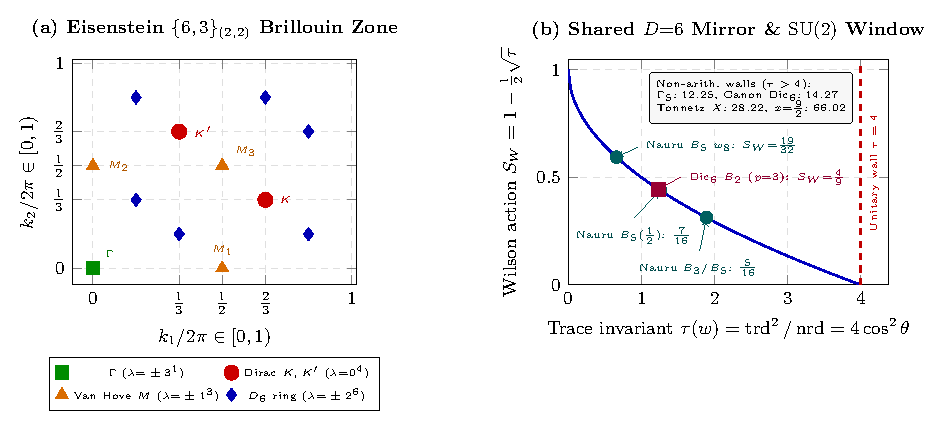
\includegraphics[width=\textwidth]{figures/fig5_eisenstein_hurwitz_mirror.pdf}
\caption{(a)~$12$ dual Bloch momenta of the Eisenstein honeycomb $\{6,3\}_{(2,2)}\cong\GP(12,5)$ on $\Z[\omega]/(2(1-\omega))$ hitting graphene Dirac points $K,K'$ ($\lambda=0^4$) and Van Hove $M$-points ($\lambda=\pm 1^3$). (b)~Shared-discriminant $D=6$ dual-prime mirror and compact $\SU(2)$ Wilson action $S_W(w)=1-\tfrac12\sqrt{\tau(w)}$ separating all four definite arithmetic uniformizations from all four non-arithmetic hyperbolic walls ($\tau>4$).}
\label{fig:eisenstein_mirror}
\end{figure}

To quantify the rarity of Nauru's simultaneous spectral gap ($\lambda_{\mathrm{nt}}=2.000$) and girth ($6$) against generic $24$-vertex $3$-regular bipartite graphs, Gate~P1 executes a keyed SplitMix64 randomized control sweep ($N=200$, seed \texttt{0x2ad1caa0125}, bit-exact replay verified): random controls yield mean $\lambda_{\mathrm{nt}}=2.5673$, minimum $\lambda_{\mathrm{nt}}=2.3248$, $197/200$ Ramanujan, $1/200$ with girth $\ge 6$, and \textbf{$0/200$} matching or beating Nauru's $\lambda_{\mathrm{nt}}=2.000$. Table~\ref{tab:comparison} synthesizes the complete shared-discriminant $D=6$ dual-prime arithmetic landscape.

\begin{table}[t]
\centering\scriptsize\setlength{\tabcolsep}{2.0pt}
\caption{Head-to-head shared-discriminant $D{=}6$ dual-prime synthesis: Tonnetz $X$ (Paper~\#01) vs.\ Nauru $Y$ ($B_3, p{=}2$) vs.\ $\mathrm{Dic}_6$ twin $Z$ (Hurwitz $B_2, p{=}3$).}
\label{tab:comparison}
\begin{tabular}{llll}\toprule
Invariant & Tonnetz $X$ \cite{ergentics2026pc} & Nauru $Y=\GP(12,5)$ & $\mathrm{Dic}_6$ Twin $Z$ \\\midrule
Tree & $T_3$ ($\PGL_2(\Q_2)$) & $T_3$ ($\PGL_2(\Q_2)$) & $T_4$ ($\PGL_2(\Q_3)$) \\
Lattice / $g$ & $\{6,3\}_{(4,2)}$ ($g{=}13$) & $\{6,3\}_{(2,2)}$ ($g{=}13$) & $4$-reg.\ ($g{=}25$) \\
Girth & $6$ & $6$ ($0$ $4$-cycles) & $4$ \\
$\lambda_{\mathrm{nt}}$ vs.\ Ram. & $\sqrt{5}\approx 2.236 < 2\sqrt{2}$ & $\mathbf{2.000}<2\sqrt{2}$ ($+30.9\%$) & $\mathbf{3.000} < 2\sqrt{3}$ \\
$\F_p$ Weil & Octic ($g\ge 5$ req.) & \textbf{All $5/5$ $\F_2$-ell.} & $\F_3$-ell.\ + $4{\times}g{=}2$ \\
Raynaud $|K|$ & $2^{15}\cdot 3^2\cdot 23^2$ & $\mathbf{2^7\cdot 3^4\cdot 5^6}$ & $2^{12}\cdot 3\cdot 5^2\cdot 7^2\cdot 13^4$ \\
Gonality & $6$ (non-reduced) & $\mathbf{6}$ (prime hex) & $\mathbf{8}$ (2-coset) \\
$|\Aut(C)|$ & $24$ & $\mathbf{144=12(g-1)}$ & $\mathbf{96=4(g-1)}$ \\
Arithmetic / $\Q$ & No ($\tau{=}\frac{7225}{256}{>}4$) & \textbf{Yes: $B_3$ ($6$), $B_5$ ($10$)} & \textbf{Yes: $B_2$ ($6, p{=}3$)} \\
$\SU(2)$ $S_W$ & Non-unitary ($\tau{>}4$) & $\mathbf{5/16,\; 7/16,\; 19/32}$ & $\mathbf{4/9}$ ($\tau{=}100/81$) \\
Tower & --- & Cong.\ ($\tfrac52$); non-cong.\ $V_4$ ($\tfrac12,\tfrac32$) & Non-cong.\ $C_3$ ($K_{4,4}$) \\
Borel $X_0^D(N)$ & $0/19$ ($2$-adic) & $0/19$ (\texttt{NEG-M18}) & $0/19$ (\texttt{NEG-M20}) \\\bottomrule
\end{tabular}
\end{table}

\subsection*{Data, code, and formal proof availability}
All results are reproducible from first principles inside \path{papers/triadic_wreath_nauru/}: pure Python ($15/15$ gates, \path{code/triadic_nauru_verify.py}, SHA-256 calibration \path{data/triadic_nauru_calibration.json}), zero-Mathlib Lean~4.36.0 ($37/37$ theorems, \path{lean/TriadicNauru/Core.lean} and \path{SnfCertificates.lean}), and zero-crate Rust ($11/11$ integration tests, $10/10$ core suites, \path{rust/}), continuously audited by \path{tests/content_integrity_audit.py}. Refuted hypotheses and scope boundaries are permanently logged in \path{NEGATIVES.md} (\texttt{NEG-M15}--\texttt{NEG-M23}).

\bibliographystyle{amsplain}
\bibliography{references}
\end{document}
